%------------------------------------------------------------------------------%
%Praca magisterska
%Modele rynkowe Inflacji
%Mateusz Golatowski
%------------------------------------------------------------------------------%
\documentclass{mini}
\usepackage[utf8]{inputenc}
\usepackage{graphicx} 
\usepackage{caption}
\newcommand{\hilight}[1]{\colorbox{yellow}{#1}}
%\numberwithin{equation}{chapter}
\setlength{\parindent}{10mm}
%------------------------------------------------------------------------------%
\title{Modele rynkowe inflacji}
\author{Mateusz Golatowski}
\supervisor{dr inż. Mariusz Niewęgłowski}
\type{magisters}
\discipline{matematyka}
\monthyear{kwiecień 2018}
\date{\today}
\album{237430}
%------------------------------------------------------------------------------%
%\linespread{1.3}

\theoremstyle{mythstyle}
\newtheorem{Twierdzenie}{Twierdzenie}[chapter]
\newtheorem{Definicja}{Definicja}[chapter]
\newtheorem{Stwierdzenie}{Stwierdzenie}[chapter]
\newtheorem{Lemat}{Lemat}[chapter]
\newtheorem{Fakt}{Fakt}[chapter]
\newtheorem{Wniosek}{Wniosek}[chapter]
\newtheorem{Uwaga}{Uwaga}[chapter]
%------------------------------------------------------------------------------%

\begin{document}
\maketitle
\tableofcontents

\chapter*{Wstęp}
%	% Cel pracy,  wyzwania związane z ryzykiem inflacyjnym
%	% postawienie problemu, cel i główne pytania
%	
%	Temat aktualny i niezwykle ważny. Inflacja - jak ją modelować i jak się przed nią zabezpieczać?
%	
%	
%	W ostatnich latach w większości krajów rozwiniętych dominowały niskie wskaźniki inflacji. Przyczyny? Spadające ceny surowców, niskie moce produkcyjne, wysoka stopa inflacji
%	
%	Aktualnie przewiduje się, że zmieni się to - na świecie widoczny jest wzrost oczekiwań inflacyjnych. Wskazują na to wzrosty cen surowców energetycznych oraz metali przemysłowych (miedzi, aluminium, cynku i węgla) a także zmiany polityczne w szczególności w Stanach Zjednoczonych oraz Wielkiej Brytanii.
%	
%	Jak się przed nią bronić? 
%	
%	Inwestycja w nieruchomości i metale szlachetne, a w szczególności w złoto, które jest jednym z niewielu aktywów dobrze dywersyfikującym portfele. Inwestycja w nieruchomością może chronić przed inflacją, ponieważ zazwyczaj ceny wynajmu idą w górę wraz z tempem wzrostu cen.
%	Inwestowanie w instrumenty finansowe, których wycena wzrasta wraz z rosnącą inflacją (obligacje indeksowane inflacją, swapy inflacyjne), czyli instrumenty, których nominał, od którego naliczane jest oprocentowanie jest indeksowany o wskaźnik inflacji (niestety, w Polsce mamy niską płynność takich instrumentów)
%	
%	Wzrost ilości gotówki poprzez zwiększenie ilości pieniądza papierowego lub wydobycia złota w obiegu prowadzi do nagłego spadku jego wartości i wzrostu cen. Oznacza to, że w miarę upływu czasu koszty usług i towarów wzrasta, zaś siła nabywcza pieniądza spada. Taki zmiany w gospodarce mierzone sa za pomocą wskaźnika cen konsumpcyjnych (Consumer Price Index - CPI). Uwzględnienie spadku siły nabywczej jest niezwykle ważne w przypadku systemów emerytalnych, gdzie indeksacja do wskaźnika inflacji gwarantuję,  że realna wartość przyszłych wypłacanych świadczeń nie będzie spadać w czasie.
%		
%	Obecnie fundusze inwestują pieniądze w akcje, obligacje i nieruchomości. Z nich pokrywają później przyszłe zobowiązania, które obejmują głównie emerytury. 
%	...
%		
%	Celem niniejszej pracy jest przedstawienie metodologi modelowania inflacji i powiązanych z nią pochodnych instrumentów. Pozwoli to na sformułowanie podejścia do wyceny instrumentów pochodnych inflacji i opisanie najbardziej popularnej metody, która jest używana także przy wycenianiu waluty obcej oraz pochodnych stóp procentowych. Najwygodniejszym sposobem myślenia o inflacji jest utożsamianie go z indeksem cen konsumpcyjnych (CPI) jako ceny waluty obcej. Takie podejście jest uznawana za jak najbardziej słuszne i jest powszechnie stosowane.
%			
%	Punktem wyjścia jest rozważenie rynku rządowych obligacji i obligacji indeksowanych inflacją. Indeksowanie odbywa się w odniesieniu do wskaźnika cen konsumpcyjnych. Definiujemy go jako tempo przeciętnego wzrostu ogólnego poziomu cen tych samych towarów i usług. \\
%		
%	Pytanie i wyzwania związane z ryzykiem inflacyjnym
%		
%	W jaki sposób mierzyć i modelować inflację na rynku?
%	Jakie rodzaje produktów ideksowanych do wskaźników inflacyjnych są dostępne?
%	Jak wyceniać instrumenty inflacyjne?
%	..
%	1. Jakie probelmy w pracy/tematy/główne tezy/zakres pracy/matody/techniki/dlaczego taki temat
%	2. najwazniejsze pozycje bibliograficzne/ trzy najważnejsze źródła
%	3. uzasadnienie podziału pracy na rozdziały/co w poszczególnych rozdziałach/dalczego taki układ
%	4. jakie typy źródeł i dlaczego z nich/metody badań/
	
\chapter{Inflacja}
	
	\section{Rynek inflacji}
	
	Według klasycznej definicji inflacja jest procesem wzrostu przeciętnego poziomu cen usług i towarów w gospodarce. Jego skutkiem jest spadek siły nabywczej pieniądza. Na poziom inflacji wpływa polityka pieniężna banku centralnego, który jest nadrzędnym organem odpowiadającym za pomiar i ocenę ogólnego poziomu cen. Procesem przeciwnym jest deflacja, czyli ogólny spadek cen.
	
	Samo zjawisko inflacji jest jednym z elementów, który nie można pominąć przy modelowaniu rynków finansowych. W obecnych czasach rozwoju gospodarczego i technologicznego obserwujemy szybsze tempo przepływów pieniężnych a więc wzrost szybkości cyrkulacji pieniądza. Dodatkowo następuje zwyżka podaży pieniądza emitowanego, która odbywa się poprzez zwiększenie ilości pieniądza papierowego w obiegu. Prowadzi to do nagłego spadku jego wartości i wzrostu cen. Skutkuje to także zwiększaniem się zadłużenia i jedynie częściowym wpływem środków do gospodarki. Oznacza to, że w miarę upływu czasu koszty usług i towarów wzrastają, zaś siła nabywcza pensji i oszczędności spada.
	
	Wzrost ilości pieniądza w obiegu może spowodować nagły spadek jego wartości i gwałtowny wzrost cen towarów. Jest to jeden z przykładów powstawania inflacji. Ekonomiści podejmują próby znalezienia innych przyczyn. Prowadzi to powstawania wielu teorii dotyczących tego zagadnienia. Oprócz przykładu podanego wcześniej, istotną rolę odgrywa popyt i podaż. Jeśli popyt wzrasta szybciej niż podaż, powoduje to znaczny wzrost cen towarów i usług, a zatem inflację. Inną przyczyną powstawania inflacji jest wzrost wynagrodzeń pracowników, który łączy się z podniesieniem cen produktów. W krajach rozwijających się umiarkowana inflacja może świadczyć o dobrej koniunkturze, jednak z drugiej strony może działać niekorzystnie w szczególności, jeśli nie jest brana pod uwagę w zarządzaniu ryzykiem portfeli inwestycyjnych.
	
	Uwzględnienie spadku siły nabywczej pieniądza jest niezwykle ważne w przypadku systemów emerytalnych, gdzie zabezpieczenie w postaci indeksacji do wskaźnika inflacji gwarantuje, że realna wartość przyszłych wypłacanych świadczeń nie będzie istotnie spadać w czasie. Instrumenty powiązane z inflacją (ang. Inflation Linked Products, ILP) takie jak obligacje indeksowane do inflacji (ang. Inflation Linked Bonds, ILB) oraz instrumenty pochodne powiązane z inflacją oferują rozwiązania, dzięki którym możemy bezpośrednio zabezpieczyć się przez ryzykiem związanym ze wzrostem inflacji. Wykorzystanie tych instrumentów gwarantuje utrzymanie stabilnego poziomu siły nabywczej pieniądza w czasie.
		
	Sam rynek instrumentów pochodnych inflacji wzrósł z prawie nieistniejącego poziomu i dość egzotycznej gałęzi gospodarki do elementu o dużym potencjale wzrostu. Tempo tego wzrostu było bardzo szybkie. W 2012 wielkość transakcji na samym rynku obligacji inflacyjnych wzrosła do 2 000 mld dolarów (ponad dziesięciokrotnie więcej w porównaniu z rokiem 2002, żródło Lazard Research). Rozrost tej gałęzi rynku w ciągu ostatnich kilku lat wynika częściowo z korzystnej sytuacji makroekonomicznej. Niskie zyski z tradycyjnych produktów o stałym dochodzie i niechęć ze strony inwestorów do podejmowania ryzyka w formie innych aktywów doprowadziły do gwałtownego wzrostu popytu na produkty strukturyzowane. Rynek produktów powiązanych z inflacją szybko rośnie i stanowi ok 2\% części rynku nominalnych kontraktów wymiany stóp procentowych. 
		
	Inflacja mierzona jest za pomocą wskaźnika cen towarów i usług konsumpcyjnych w gospodarce. Pod względem indeksów inflacji, rynek instrumentów pochodnych w dużej mierze skupia się na tych samych wskaźnikach, jak na rynku rządowych obligacji indeksowanych do inflacji. Głównym wskaźnikiem inflacji na rynku europejskim jest indeks HICPxT z Eurostatu, na rynku francuskim  indeks FRCPI z INSEE, na rynku brytyjskim wykorzystywany jest indeks RPI, a na rynku amerykańskim indeks CPI.
		
	\section{Rys historyczny}
		
	Praktyka powiązania płatności odsetek od obligacji z indeksacją jest stosunkowo stara. Już w 1742 roku w stanie Massachusetts w USA wprowadzono rachunki związane z ceną srebra na London Exchange. W czasie rewolucji amerykańskiej, żołnierzom zostały wydawane szczególne papiery wartościowe - snoty dewaluacyjne. Dzięki nim mogli oni zachować realną wartość wynagrodzenia. Indeksacja kontraktów do pojedynczego towaru stała się istotna dopiero później, w momencie gdy gwałtownie wzrosła cena srebra. W związku z tym w 1780 roku zostały wyemitowane obligacje, które pozwalały na zachowanie realnej wartości wynagrodzenia dla żołnierzy. Pod uwagę wzięto wtedy najbardziej popularny koszyk dóbr spożywczych: pięć buszli kukurydzy, sześćdziesiąt osiem i cztery siódme funtów wołowiny, dziesięć funtów owczej wełny i szesnaście funtów jeleniej skóry. Produkty finansowe zabezpieczające przed wzrostem inflacji były jednak zbyt trudne dla zrozumienia dla ludzi bez wykształcenia ekonomicznego lub matematycznego, dlatego nie cieszyły się dużą popularnością.
		
	W czasach obecnych obligacje indeksowane do inflacji po raz pierwszy zostały wydane na międzynarodowych rynkach kapitałowych przez Izrael w 1955r. Ich rozwój rozszerzył się na całym świecie i produkty te zostały zintegrowane w wielu portfelach. Celem ILB (ang. Inflation Linked Bonds) jest zapewnienie zabezpieczenia siły nabywczej przez bezpośrednie powiązanie papieru wartościowego z indeksem inflacji przez cały okres życia obligacji. Kontrakty te zawierają dwie formy płatności: realną stopę procentową ustanowiona na początku okresu i rekompensatę za utratę siły nabywczej. W kontraktach ILB realny dochód w okresie ich trwania jest pewny, natomiast dochód nominalny jest zdeterminowany ex post. Tak więc klasa aktywów ILB i ich pochodnych daję szeroką gamę okazji dla inwestorów do ochrony przed inflacją.  
		
	W XX wieku wiele państw doświadczyło wysokiej inflacji. Było to głównym powodem wyemitowania pierwszych obligacji indeksowanych inflacją jako zabezpieczenia dla długoterminowych kontraktów. Rząd UK w 1981 rozpoczął program wydawania ILB a zaraz po nim Australia w 1985, Kanada w 1991, Szwecja w 1994, USA w 1997, Francja w 1998, Włochy w 2003, Japonia w 2004 oraz Niemcy w 2006r. W większości to właśnie rządy państw emitowały papiery wartościowe indeksowane inflacją. Z czasem podobne kontrakty zaczęły wprowadzać do obiegu także większe korporacje.
	
	\begin{figure} [h]
		\centering
		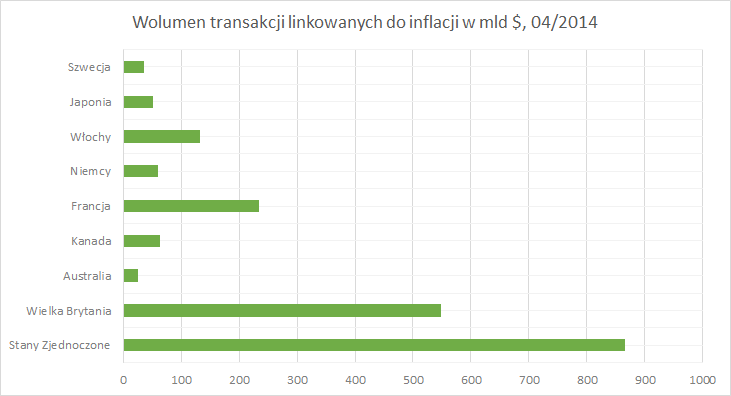
\includegraphics[scale=0.8]{graphics/wolumen.png}
		\caption{Wolumen transakcji zawieranych na największych rynkach produktów inflacyjnych na świecie.}
	\end{figure}

	\section{Uczestnicy rynku}
		
	Produkty indeksowane inflacją mogą przyciągnąć różne grupy inwestorów, takich jak: banki, fundusze emerytalne, fundusze inwestycyjne, firmy ubezpieczeniowe czy fundusze hedgingowe. Dla przykładu bank zajmie pozycję otrzymującą dany poziom inflacji w celu zabezpieczenia produktów hipotecznych powiązanych z inflacją. Z kolei firmy ubezpieczeniowe i fundusze emerytalne inwestują pieniądze w akcje, obligacje i nieruchomości. Z nich pokrywają później przyszłe zobowiązania, które obejmują głównie emerytury i świadczenia. Aktywa ILB (ang. Inflation Linked Bonds) stanowią idealne dopełnienie, które pozwala zabezpieczyć ich długoterminowe pozycje inwestycyjne.

	W ostatnich latach rynek produktów indeksowanych urósł niezwykle szybko również na wschodzących rynkach kapitałowych (Brazylia, Meksyk, Turcja, Południowa Afryka). Ponadto odbyło się kilka emisji przez prywatnych emitentów, głównie banków i funduszy emerytalnych.

	\section{Zarządzanie ryzykiem}
	
	Inflacja jest także istotnym czynnikiem, który powinien zostać uwzględniony w obszarze zarządzania ryzykiem. Niemal każda decyzja finansowa podejmowana przez organizację i prywatnych inwestorów wiąże się z podejmowaniem szeregu różnych ryzyk. Zarządzanie ryzykiem ma na celu stosowanie zasad i metod, które pozwalają kontrolować i optymalizować ryzyko finansowe w szczególności jeśli dotyczy ono inwestycji długoterminowych. Ryzyko operacji na rynkach finansowych może przyjmować wiele form i mieć odmienne źródła pochodzenia. W ramach obszaru  ryzyka rynkowego związanego ze zmiennością na rynkach finansowych można wyróżnić ryzyko inflacji, które występuję w momencie, gdy zmienia się siła nabywcza dochodu z inwestycji. Identyfikacja i ocena wpływu efektu tego ryzyka jest w szczególności istotna w przypadku pozycji inwestycyjnych o wieloletnim terminie zapadalności i w ramach zarządzania powinna zostać w odpowiedni sposób zabezpieczona. Ochronę przed negatywnymi skutkami inflacji zapewniają odpowiednio dobrane instrumenty pochodne, które w szczegółowy sposób zostaną opisane w poniższej pracy.
	
\chapter{Modelowanie inflacji}

	W rozdziale drugim zostały przedstawione właściwe podejście do modelowania procesu inflacji. Wprowadzono w tym celu podział na ujęcie nominalne i rzeczywiste. W dalszej części przedstawiono wskaźnik cen konsumpcyjnych a także omówiono metody tworzenia krzywej projekcyjnej indeksu zmiany cen.
	
	\section{Indeksacja}
	
	Porównując kwoty pieniądza pochodzące z różnych okresów wykorzystujemy wskaźniki cen, aby usunąć skutki inflacji. Korygując wartości  o wybrany indeks inflacji stosujemy indeksację (ang. indexed).\\
	
	\begin{Definicja}
		Indeksacją nazywamy zmianę wartości jednostki pieniądza dokonywaną automatycznie na mocy umowy prawnej mającą na celu uwzględnienie skutków inflacji.
	\end{Definicja}

	W dalszej części pracy o indeksacji będziemy mówić w kontekście instrumentów finansowych indeksowanych do inflacji, w których nominał, od którego naliczane jest oprocentowanie, jest indeksowany do wskaźnika inflacji.
	
	\section{Stopa nominalna, rzeczywista i inflacja}
	
	Uwzględniając przepływy finansowe następujące w różnych okresach czasu możemy podejść do ich analizy w sposób nominalny lub rzeczywisty. Pierwszy z nich jest podejściem standardowym i zakłada odniesienie się do cen lub stóp zwrotu w kategorii ich nominalnych wartości. Zakładamy, że jednostka pieniądza jest niezmienna w czasie i nie rozpada się ze względu na spadek jej siły nabywczej. Nominalne stopy przedstawiają stawki w kategorii wartości pieniądza ale nie w znaczeniu siły nabywczej. Jeżeli uwzględnimy proces inflacji otrzymamy rzeczywistą wartość pieniądza i realne stopy a także będziemy mogli rozważać jaką realną wartość mają nasze oszczędności lub kapitał inwestycyjny. Odróżnienie nominalnego i realnego podejścia jest szczególnie istotne w przypadku inwestycji długoterminowych. Inwestorzy myśląc o wartości kapitału i późniejszych potencjalnych zyskach, bardzo często ignorują wpływ inflacji i zmianę siły nabywczej pieniądza w czasie. Przykład obrazujący dany problem został przedstawiony poniżej.
	
	Załóżmy, że jesteśmy zainteresowani kupnem amerykańskiej obligacji jednorocznej o oprocentowaniu 8\%. Opisując inwestycję w prosty sposób: dziś płacimy 100\$ za rok mamy zagwarantowaną wypłatę równą 108\$, podchodzimy do problemu nominalnie - patrzymy na wartości pieniądza, działamy stopą nominalną, nie bierzemy pod uwagę innych czynników. 
			
	Dodatkowo zakładamy, że stopa inflacji przez najbliższy rok będzie  wynosiła 4\%. Oznacza to, że wybrany koszyk dóbr, dziś nominalnie wart 100\$ za rok będzie kosztował 104\$. Jeśli wypłatę z obligacji będziemy chcieli przeznaczyć i wydać na wybrany koszyk dziś zapłacilibyśmy za niego 100\$ a za rok już 104\$. W momencie zapadalności obligacji dostajemy nominalnie 108\$ jednak za tą samą cenę w porównaniu z poprzednim rokiem możemy kupić już mniej. Realna wartość naszej inwestycji uwzględniająca zmianę wartości pieniądza w czasie będzie zatem równa 108\$ - 104\$ = 4\$.\\
		
	\begin{Definicja}
			Nominalną stopą procentową (ang. nominal interest rate) nazywamy stopę, zgodnie z którą bank nalicza odsetki.
	\end{Definicja}

	Stopa nominalna zazwyczaj obrazuje informacje z rynku i nie jest skorygowana o skutki zmiany wartości pieniądza w czasie. Stopa realna obrazuje jak zmienia się siła nabywcza pieniądza.\\
	
	\begin{Definicja}
		Realną stopą procentową (ang. real interest rate) nazywamy stopę procentową skorygowaną o skutki inflacji.
	\end{Definicja}

	Związek pomiędzy zmianą poziomu cen i stóp procentowych opisuje uproszczone równanie Fishera [8], zgodnie z którym
	\begin{eqnarray}
		r = n - i
	 \end{eqnarray}
	gdzie $r$ oraz $n$ oznaczają odpowiednio realną i nominalną stopę zwrotu zaś $i$ inflację. Realna stopa procentowa stanowi różnicę nominalnej stopy procentowej i stopy inflacji. Jeśli inflacja jest dodatnia, to realna stopa jest mniejsza od nominalnej. Jeżeli mamy do czynienia z procesem odwrotnym do inflacji, czyli spadkiem cen - deflacją - stopa nominalna będzie większa niż rzeczywista. 
	
	\section{Wskaźnik cen konsumpcyjnych}
		
	 Wskaźnik cen konsumpcyjnych (ang. Consumer Price Index, CPI) lub indeks cen konsumenta jest najczęściej używaną miarą wykorzystywaną do pomiaru poziomu cen dóbr i usług kupowanych przez typowego nabywcę. Zazwyczaj raz w miesiącu biuro statystyczne odpowiednie, dla każdego kraju publikuje informacje o wartości wskaznika cen. Jego wartość jest podstawą do wyznaczenia stopy inflacji.\\
	 
	 \begin{Definicja}
	 	Stopą inflacji nazywamy wyrażoną w procentach zmianę wskaznika cen dla danego okresu w porównaniu z rokiem poprzednim.
	 \end{Definicja} 
	 	 
	 Wielkość inflacji mierzona jest jako procentowy wzrost wybranego wskaźnika zmiany cen usług i towarów. Samych wskaźników istnieje wiele a wybór odpowiedniego jest jednym z elementów odpowiedniej strategii inwestycyjnej uwzględnianych przez inwestorów. Przykładowe najpopularniejsze indeksy inflacyjne wraz z krajami występowania zostały przedstawione w tabeli poniżej
	
	\begin{center}
		\begin{tabular}{c  c c}
			\textbf{Indeks} & \textbf{Waluta}  \\ \hline
			US CPI Urban NSA & USD \\
			UK RPI & GBP \\
			HICP (Harmonised Index of Consumer Prices) & EUR \\
			France HICP ex-tobacco & EUR \\
			German Euroland HICP ex-tabacco & EUR  \\
			CPI & PLN \\
		\end{tabular}
%	\caption{Przykładowe indeksy inflacyjne wraz z dopasowaną walutą.}
	\end{center}

	\section{Konwencja indeksowania}
	
	W standardowej konwencji instrumenty finansowe indeksowane do inflacji używają wartości indeksu cen - indeksu referencyjnego (ang. Reference Index). Praktycznie jest on powiązany z indeksem wzrostu cen za dany miesiąc (odnoszący się do pierwszego dnia miesiąca), a wartość wskaźnika jest ustalone z odpowiednim opóźnieniem (zazwyczaj opóźnienie jest równe trzem miesiącom).\\
	
	\begin{Definicja}
		Indeksem referencyjnym (ang, Reference index) nazywamy wybrany indeks wzrostu cen (inflacji) odpowiadający ustalonemu miesiącowi
	\begin{eqnarray*}
		Reference\_Index = Price\_Index(m),
	\end{eqnarray*}
	gdzie $m$ oznacza ustalony miesiąc.\\
	\end{Definicja}

	\begin{Uwaga}
	Może się też zdarzyć, że instrument wykorzystuje indeks referencyjny powiązany z inną datą niż data płatności. Dla przykładu w standardowej miesięcznej konwencji instrument finansowy, dla którego następuje przepływ w 4 dniu listopada (ang. payment date) z ustalonym opóźnieniem indeksu równym trzem miesiącom wykorzysta wartość indeksu z sierpnia. 
	\end{Uwaga}

	\section{Interpolacja indeksu}
	
	W przypadkach niestandardowych wartość współczynnika inflacji jest interpolowana liniowo pomiędzy dwoma miesiącami i wykonywana dla wartości w miesiącu płatności. Końcowa wartość współczynnika wzrostu cen wyznaczana jest następująco
	\begin{eqnarray*}
		Reference\_Index = Price\_Index(m_1) + \bigg(\frac{d - 1}{D}\bigg) \bigg(Price\_Index(m_2) - Price\_Index(m_1)\bigg),
	\end{eqnarray*}
	gdzie $d$ oznacza dzień miesiąca daty terminu płatności, zaś $D$  liczbę dni kalendarzowych w miesiącu płatności. Referencyjny indeks dla daty startu transakcji jest obliczany w ten sam sposób przy zastosowaniu daty rozpoczęcia transakcji.
	
	\section{Notacja indeksu}
	
	Określamy, że wartość referencyjnego indeksu cen będziemy oznaczać symbolem $I(t)$ dla $t \le T^*$, gdzie $T^*$ to ustalony horyzont czasowy. Oznacza to, że będąc w chwili czasu $t$ równej dacie 2016/11/20 i zachowując standardową konwencję opóźnienia trzymiesięcznego oraz wartości indeksu z początku miesiąca (nieinterpolowaną) wartość referencyjnego indeksu będzie równa
	\begin{eqnarray*}
		I(t) = Price\_Index(Sierpien2016).
	\end{eqnarray*}
	W poniżeszj tabeli przedstawiono standardowe konwencje kwotowań swapów zerokuponowych
	\begin{center}
		\begin{tabular}{c c c c}
			\textbf{Obszar} & \textbf{Indeks}  & \textbf{Opóźnienie} & \textbf{Konwencja}\\ \hline
			Strefa Euro & HICPexT & 3M & Miesięczna \\
			USA & CPI & 3M & Interpolacja \\
			Wielka Brytania & UK RPI & 2M/8M & Miesięczna \\
			Kanada & CPI & 3M & Miesięczna \\
			Australia & HICPxT & 6M & Miesięczna \\
			Francja OATi & French CPIxT & 3M & Miesięczna \\
			Francja OATei& HICPxT & 3M & Miesięczna \\
			Niemcy & HICPxT & 3M & Miesięczna
		\end{tabular}
	\end{center}
	
	\section{Detale techniczne}
	
	W celu zrozumienia obrotu i wyceny ILP (ang. Inflation Linked Products) istotne jest zwrócenie uwagi na dwa punkty: obliczanie wskaźnika indeksu oraz ochrona przed deflacją. Wskaźnik indeksu jest obliczany codziennie przez emitenta i udostępniany do obrotu (agencje: Bloomberg, Reuters). Ważną kwestią przy obliczaniu inseksów jest wybranie wskaźnika inflacji. W przypadku USA jest to wskaźnik cen konsumpcyjnych CPI, w Wielkiej Brytanii wskaźnik cen detalicznych RPI, Francja ma obligacje powiązane z CPI ex-tabacco jak i inne z HICP ex-tabacco. \\
		\begin{figure} [!h]
		\centering
		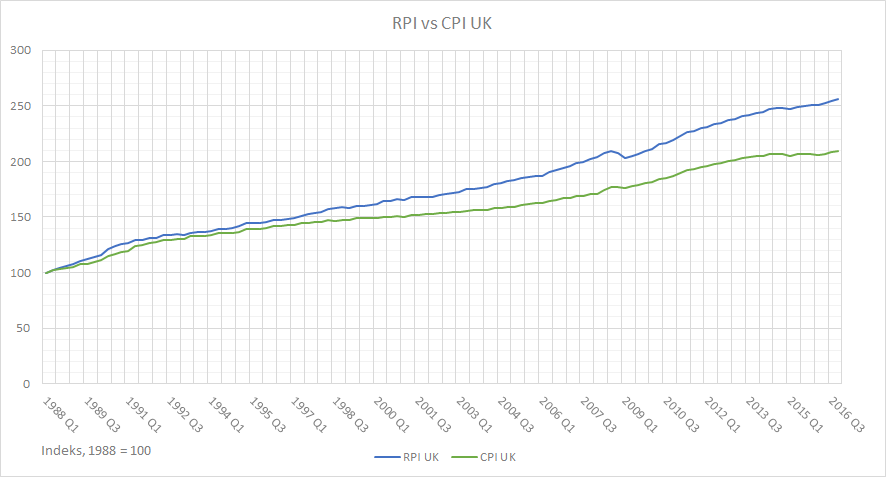
\includegraphics[scale=0.65]{graphics/rpivscpi.png}
		\caption{Wykres historycznych kwotowań indeksu RPI oraz CPI w Wielkiej Brytanii.}
	\end{figure}

	\begin{Uwaga}
			Instrumenty finansowe ILP zawsze są połączone z ustalonymi wskaźnikami, a te ze względu na różne konstrukcje powodują, że dane ustalone zabezpieczenie może gwarantować różne poziomy ochrony siły nabywczej pieniądza.
	\end{Uwaga}

	Właściwą ochronę przed inflacją inwestor może uzyskać dopiero, jeżeli weźmie pod uwagę metodykę uzyskiwania składu koszyka i obliczania wartości dla danego wskaźnika zmiany cen. Należy rozważyć czy wybrane zabezpieczenie oferuję realną ochronę i czy bazowy indeks cen nie podlega manipulacji poprzez np. holistyczne podejście do kalkulacji wskaźników cen. Dla przykładu w Stanach Zjednoczonych poprawa jakości produktów jest zawarta w obliczaniu indeksu co może spowodować "sztuczne" zaniżenie inflacji. W Wielkiej Brytanie z kolei trwa dyskusja dotycząca wyboru między wskaźnikami RPI a CPI, która wynika z zasadniczych różnic we wzorach w długim okresie z powodu dodatkowych kosztów wynajmu i odsetek. \\ 
	\begin{Uwaga}
		Wskaźniki inflacji nie są obliczane każdego dnia lecz za okres jednego miesiąca i publikowane z opóźnieniem czasowym. W zależności od wybranego indeksu, "bieżąca" wartość zostaję podana od jednego do trzech miesięcy później. Kalkulacja wskaźnika inflacji zależy od szczegółowych przepisów w odniesieniu do których poziom indeksu odniesienia jest traktowany jako "bieżący" (indeksacja opóźnienia).
	\end{Uwaga}

	Oddzielnym czynnikiem, który należy wziąć pod uwagę jest fakt, że obligacje różnią się procedurą podejścia do zjawiska przeciwstawnego - deflacji. Przykładem może być Japonia, w której spadek cen w dłuższych okresach czasu może spowodować, że wskaźnik spadnie poniżej jednostki. W takiej sytuacji kupon nominalny jest mniejszy niż kupon rzeczywisty lub wartość nominalna obligacji spadnie poniżej 100. W wielu krajach (USA, Francja, Włochy, Szwecja) istnieje zabezpieczenie przed takim zjawiskiem poprzez nałożenie ograniczenia dolnego, gdzie wartość nominalna obligacji nie może spaść poniżej 100. Wprowadzenie takiego zabezpieczenia stanowi wbudowaną opcję,która powinna zostać uwzględniona przy wycenie instrumentu. Ponadto w przypadku obligacji korporacyjnych należy pamiętać o włączeniu do wyceny premii związanej z ryzykiem kredytowym kontrahenta (ryzykiem niedotrzymania warunków umowy) i płynności (ryzyko braku płynności instrumentu występuje jeśli warunki rynkowe uniemożliwiają dokonanie transakcji kupna/sprzedaży danego instrumentu). Standardem w przypadku obligacji komercyjnych jest także wbudowana opcja przedwczesnego wykupienia obligacji przez emitenta. W praktyce rynkowej cenę każdej z powyższych wbudowanych opcji wyraża się w postaci czynnika korygującego (ang. Option Adjusted Spread) oraz  spreadu związanego z ryzykiem kredytowym i płynności, który jest dodawany do faktora dyskontującego przyszłe przepływy. W tej pracy będziemy rozważać jedynie wyceny bez uwzględnienia powyższych opcji i ryzyk.
			
	\subsection{Interpolacja}
	
	Krzywa terminowa (zależność pomiędzy wielkością indeksu a terminem jego wyznaczenia w przyszłości) indeksu cen wyznaczana jest przy wykorzystaniu informacji dotyczących aktualnych kwotowań instrumentów powiązanych inflacją, które notowane  są zazwyczaj w odstępach rocznych lub kilkuletnich. Dostępne na rynku są kwotowania o następujących terminach zapadalności: 1Y, 2Y, 3Y, 4Y, 5Y, 6Y, 7Y, 8Y, 9Y, 10Y, 12Y, 15Y, 20Y, 25Y, 30Y, 40Y, 50Y. Nie znamy jednak wartości w datach zapadalności dla każdej chwili w przyszłości, dlatego aby wyznaczyć wartości krzywej w terminach pomiędzy dostępnymi węzłami stosujemy interpolacje. Jedną z możliwych i najczęściej wykorzystywaną jest metoda interpolacji logarytmicznej. \\
	
	\begin{Definicja}
		Roczny wzrost indeksu cen $q$ w chwili $t$ definiujemy jako
		\begin{equation}
		q = ln [I(t,m + 12)] - ln[I(t,m)],
		\end{equation} 
		gdzie $m$ oznacza miesiąc (pierwszy dzień miesiąca), dla którego znana jest wartość indeksu $I(t,m)$ w chwili $t$ zaś $I(t+12,m)$ oznacza wartość indeksu cen rok później.\\
	\end{Definicja}
	
	\begin{Uwaga}
		Wówczas dla $i \in [0,11]$ kolejnych miesięcy dostajemy zinterpolowane wartości cen forward indeksu cen wyznaczamy w następujący sposób
		\begin{equation}
		I(t+i,m) = I(t,m) * \exp\bigg(\frac{i*q}{12}\bigg).
		\end{equation}
	\end{Uwaga}
	
	Metodę te możemy w łatwy sposób zastosować dla przypadków, jeśli różnica pomiędzy kursami forward jest większa niż jeden rok, pamiętając o założeniu, że tempo wzrostu pomiędzy każdym miesiącem jest stałe.
	
	\subsection{Sezonowość}
	
	Jedną z cech procesu inflacji jest jej sezonowość. Oznacza to zmianę struktury ceny, która zależy od danego okresu w ciągu roku, w którym zmienia się przede wszystkim popyt na żywność i energię. Wzrost wskaźnika nie jest regularny i podlega miesięcznym wahaniom. W konsekwencji tego wskaźnik inflacji wykazuje zmiany sezonowe, które należy uwzględnić w momencie wycen instrumentów. Chcąc zbudować realistyczną krzywą indeksu cen, należy pamiętać o włączeniu sezonowej korekty.

	\begin{figure} [!h]
		\centering
		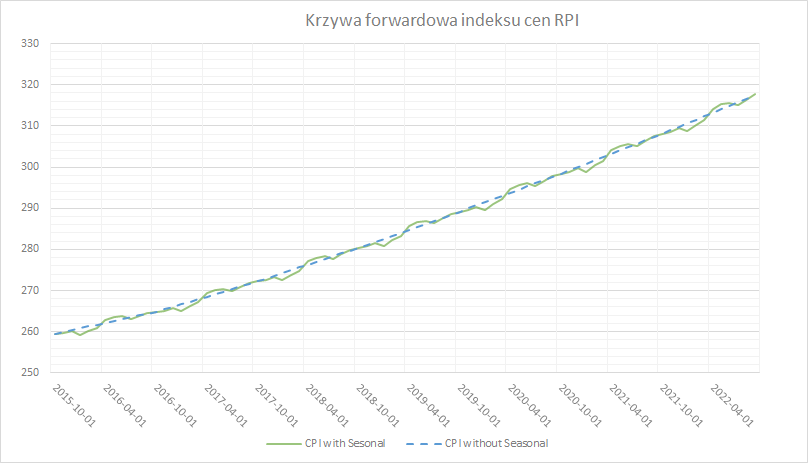
\includegraphics[scale=0.75]{graphics/rpi.png}
		\caption{Wykres krzywej forward z uwzględnieniem i bez efektu sezonowości.}
	\end{figure}
		
	\subsubsection*{Podejście multiplikatywne}
		W zależności od wyboru metody jedną z możliwości uwzględnienia wyrównania sezonowego dla indeksu cen jest zastosowanie czynników korygujących w podejściu multiplikatywnym.
		
	\begin{Definicja}
		Czynnikiem korygującym $f_i$ nazywamy wartość korekty odpowiadająca kolejnym miesiącom $m_i$ dla $i \in \{0,...,11\}$, gdzie faktor $f_0$ jest czynnikiem zmiany pomiędzy grudniem a styczniem.\\
	\end{Definicja}
	
	\begin{Definicja}
		Multiplikatywnym czynnikiem sezonowości $Adj(t,m)$ korygującym początkową wartość ceny dla roku $t$ nazywamy funkcję spełniającą równanie
		\begin{eqnarray*}
			Adj(t, m_{i+1})  = f_i * Adj(t, m_i)
		\end{eqnarray*}
	\end{Definicja}

	\begin{Uwaga}
		Korektę dla stycznia $Adj(t, m_1)$ wyznaczamy przy pomocy korekty grudniowej $Adj(t, m_0)$.\\
	\end{Uwaga}

	\begin{Uwaga}
		 Wartości czynników korygujących są wyznaczane na podstawie historycznych obserwacji przy założeniu, że skumulowana korekta sezonowości w okresie jednego roku spełnia warunek
		\begin{eqnarray*}
			\prod_{i=0}^{11} f_i = 1.
		\end{eqnarray*}
		Wówczas skorygowany indeks ceny jest równy
		\begin{eqnarray*}
			I(t,m) = Adj(t,m) * I_{notAdj}(t,m),
		\end{eqnarray*}
		gdzie $I_{notAdj}(t,m)$ jest wartością indeksu przed uwzględnieniem sezonowości.\\
	\end{Uwaga}
		
	\begin{Uwaga}
		Istnieje wiele sposobów, które można wykorzystać do konstrukcji krzywej forward: różne metody interpolacji oraz uwzględnienie lub nie czynnika sezonowości. W praktyce rynkowej dla krótszych terminów zapadalności efekt sezonowości może być bardziej istotny i należy uwzględnić go w wyznaczeniu cen. Natomiast w przypadku dłuższych terminów, sięgających nawet 40 lat efekt ten można pominąć i ograniczyć się jedynie do wyboru najlepszej metody interpolacyjnej.
	\end{Uwaga}

\chapter{Podstawy matematyki finansowej}

	W poniższym rozdziale przedstawiamy podstawowe pojęcia i twierdzenia matematyki finansowej, używane w kolejnych rozdziałach. Ustalamy horyzont czasowy $T^*$ i zupełną przestrzeń probabilistyczną $(\Omega, \mathcal{F}, \mathbb{P})$ wraz z filtracją $\mathbb{F} = (\mathcal{F}_t)_{t\in [0,T^*]}$ generowaną przez proces Wienera $W$, tzn. $\mathcal{F}_t=\mathcal{F}_t^W=\sigma(W_s:s\leq t)$ dla $t \in [0,T^*]$ ($W$ jest adaptowany do $\mathbb{F}$ oraz dla dowolnych $0 \leq s < t $ zmienna losowa $W_t-W_s$ jest niezależna od $\mathcal{F}_s$). Proces Wienera przy mierze $\mathbb{Q}$ równoważnej $\mathbb{P}$ będziemy oznaczać przez $W^\mathbb{Q}$. Zakładamy także, że obecnie znajdujemy się w chwili 0.

\section{Rachunek bankowy, obligacja zerokuponowa, kontrakt swapowy}
	Przez $B=(B_t)_{t\in [0,T^*]}$ oznaczamy proces opisujący rachunek bankowy. Zakładamy, że spełnia on następujące równanie różniczkowe
	\[ dB_t = r_t B_t dt, \ \ B_0=1, \]
	gdzie $r=(r_t)_{t\in [0,T^*]}$ jest $\mathbb{F}$-adaptowanym procesem stochastycznym określonym na $(\Omega, \mathcal{F},\mathbb{P})$, nazywanym \textit{krótkoterminową stopą procentową}.
	Rozwiązaniem powyższego równania jest proces dany wzorem
	\[ B_t = \exp\left(\int_0^t r_s ds\right), \ \ t\in [0,T^*]. \]

\begin{Definicja}
	Obligacją zerokuponową o terminie zapadalności $T$ nazywamy instrument finansowy, który gwarantuje wypłatę w wysokości 1 jednostki w danej walucie w chwili $T$. Wartość obligacji w momencie $t\in [0,T]$ oznaczamy przez $P(t,T)$.
\end{Definicja}
	W przypadku ustalonej struktury czasowej $0 \leq T_0 < T_1 <\ldots T_n$ będziemy zakładać, że dla każdego $i=1,\ldots,n$ istnieje obligacja o terminia zapadalności $T_i$.

	Na potrzeby następnych definicji zawartych w tym podrozdziale ustalmy strukturę czasową $0\leq T_0<T_1< \ldots < T_n$ i
	oznaczmy przez $\Delta_i = T_i-T_{i-1}$ długość $i$-tego okresu depozytowego, $i=1,\ldots,n$.\\

\begin{Definicja}
	Kontrakt IRS (Interest Rate Swap), lub w skrócie: swap, jest to kontrakt wymiany procentowej pomiędzy dwiema stronami, na podstawie którego w ustalonych chwilach czasu $T_1,\ldots,T_n$ strony wypłacają sobie wzajemnie odsetki od ustalonego nominału $N$  naliczane według odmiennych stóp procentowych. Jedna ze stron kontraktu dokonuje płatności odsetkowych według stopy stałej $K$, natomiast druga strona w chwilach $T_i$ dokonuje płatności według stopy zmiennej $S(T_{i-1},T_i), i=1,\ldots,n$. Stopa kontraktu IRS zostaje ustalona w momencie zawarcia kontraktu $T_0$. Strumień pieniężny złożony z płatności wyliczonych według stałej stopy nazywa się nogą stałą kontraktu IRS (ang. fixed leg), natomiast strumień płatności według zmiennej stopy -- nogą zmienną kontraktu IRS (ang. floating leg). Obie nogi kontraktu kończą się w tym samym momencie w terminie zapadalności.
	\begin{enumerate}
		\item pay-fixed IRS lub payer IRS to kontrakt IRS, którego posiadacz płaci stopę stałą i otrzymuje stopę zmienną;
		\item receive-fixed IRS lub receiver IRS to kontrakt IRS, którego posiadacz płaci stopę zmienną i otrzymuje stopę stałą.
	\end{enumerate}
\end{Definicja}
\section{Twierdzenie Girsanowa i zamiana miary}
\begin{Twierdzenie}
	Jeśli miary probabilistyczne $\mathbb{P}$ i $\mathbb{Q}$ są
	równoważne na $(\Omega, {\cal F})$, to istnieje gęstość miary $\mathbb{Q}$
	względem $\mathbb{P}$ - gęstość Radona-Nikod\'{y}ma: $\varrho = \frac{d
		\mathbb{Q}}{d \mathbb{P}}$, tzn.
	\begin{equation*}
	\mathbb{Q}(A) = \int_A \varrho d
	\mathbb{P}\ 
	\end{equation*}
	dla każdego $A \in {\cal F}$ oraz $\varrho$ jest dodatnią zmienną losową mierzalną względem ${\cal F}$.\\ 
	Ponadto zachodzi $$\frac{d \mathbb{P}}{d \mathbb{Q}} = \frac{1}{\varrho}.$$
\end{Twierdzenie}
\begin{Definicja}\textbf{Eksponenta stochastyczna}\\
	Jeśli proces $\gamma \in {\cal P}_t$, to równanie
	\begin{equation}
	dX_t = \gamma_t X_t dW_t,\quad X_0 = 1
	\end{equation}
	ma dokładnie jedno rozwiązanie nazywane eksponentą stochastyczną i jest ono zadane wzorem
	\begin{equation} \label{Dolean}
	X_t = \exp \left( \int_0^t \gamma_s dW_s - \frac{1}{2} \int_0^t
	\gamma_s^2 ds\right) = \exp \left(M_t - \frac{1}{2} \langle M \rangle_t \right),
	\end{equation} gdzie $M_t=\int_0^t \gamma_sdW_s$.\\ 
	
\end{Definicja}

\begin{Twierdzenie}\textbf{Twierdzenie Girsanowa}\\
	Niech $T < \infty$ i niech $\mathbb{Q}$ będzie miarą
	probabilistyczną równoważną $\mathbb{P}$ na $(\Omega, {\cal F}_T)$
	taką, że
	\begin{equation}
	\frac{d \mathbb{Q}}{d \mathbb{P}} = \varrho_T = \exp\left(\int_0^T \gamma_s d
	W_s - \frac{1}{2} \int_0^T \gamma_s^2 ds\right)
	\end{equation}
	dla pewnego $\gamma \in {\cal P}_T$. Jeśli $W = (W_t)_{t \in [0, T]}$ jest procesem Wienera przy mierze probabilistycznej $\mathbb{P}$ względem filtracji $\mathbb{F}$, to proces $\widetilde{W}$ zdefiniowany wzorem
	\[
	\widetilde{W}_t = W_t - \int_0^t \gamma_s ds \ \ \forall_{t \in [0,
		T]}
	\]
	jest procesem Wienera przy mierze probabilistycznej $\mathbb{Q}$ względem filtracji $\mathbb{F}$.\\
	
\end{Twierdzenie}

\begin{Wniosek}
	Przy założeniach twierdzenia Girsanowa dynamikę procesu $X_t$ można zapisać jako
	$$ dX_t = (a_t+b_t \gamma_t)dt + b_t d\widetilde{W}_t,$$
	co oznacza, że współczynnik dyfuzji nie zmienia się przy zmianie miary probabilistycznej na równoważną.\\
\end{Wniosek}
\begin{Definicja}
	\textbf{Miara martyngałowa}\\
	Miarę probbilistyczną $\mathbb{P}^*$ na $(\Omega,\mathcal{F}_T)$ równoważną mierze $\mathbb{P}$ nazywamy miarą martyngałową dla:
	\begin{itemize}
		\item zdyskontowanego procesu cen $S^*$, gdy $S^*$ jest $\mathbb{P}^*$-martyngałem względem filtracji $(\mathcal{F}_t)$,
		\item rynku $\mathcal{M}= (S,\Phi)$, gdy dla każdej strategii $\phi \in \Phi$ proces $V^*(\phi)$ zadany wzorem
		\begin{equation*}
		V^*(\phi) = \frac{V_t(\phi)}{B_t},
		\end{equation*}
		czyli zdyskontowany proces bogactwa, jest $\mathbb{P}^*$-martyngałem względem filtracji $(\mathcal{F}_t)$.\\
	\end{itemize}
\end{Definicja}
\begin{Twierdzenie}
	\textbf{Pierwsze podstawowe twierdzenie matematyki finansowej}\\
	Rynek $\mathcal{M}$ jest rynkiem bez możliwości arbitrażu wtedy i tylko wtedy gdy istnieje miara martyngałowa.\\
\end{Twierdzenie}
\begin{Twierdzenie}
	Niech $\mathcal{M}$ jest rynkiem bez możliwości arbitrażu. Wówczas cena arbitrażowa w chwili $t$ osiągalnej na rynku $\mathcal{M}$ wypłaty $X$ jest dana wzorem
	\begin{equation*}
	\Pi_{t}(X) = B_t \mathbb{E}_{\mathbb{P}^*}  \bigg( \frac{X}{B_T}\bigg|\mathcal{ F}_t\bigg)
	\end{equation*}
	dla dowolnej miary martyngałowej $\mathbb{P}^*$.\\
\end{Twierdzenie}
\begin{Definicja} \textbf{Rynek zupełny}\\
	Rynak $\mathcal{M}$ nazywamy zupełnym, gdy każda wypłata jest osiągalna na tym rynku.\\
\end{Definicja}
\begin{Twierdzenie}
	\textbf{Drugie podstawowe twierdzenie matematyki finansowej}\\
	Rynek bez możliwości arbitrażu jest zupełny wtedy i tylko wtedy, gdy istnieje dokładnie jedna miara martyngałowa.\\
\end{Twierdzenie}
\begin{Definicja}
	\textbf{Miara forward}\\
	Załóżmy, że przyjmujemy obligację zerokuponową zapadającą w chwili $T$ jako num\'{e}raire. Miarę martyngałową stowarzyszoną z tak przyjętym num\'{e}rairem nazywamy miarą forward (T-forward) i oznaczamy przez $\mathbb{P}_T$. Proces Wienera w tej mierze oznaczamy jako $W^T$.\\
\end{Definicja}
\begin{Uwaga}
	Miarę T-forward możemy zdefiniować za pomocą pochodnej Rodona-Nikod\'{y}ma wzorem
	\begin{equation*}
	\frac{d\mathbb{P}_T}{d\mathbb{P^*}} = \frac{1}{B_T P(0,T)} \   \ \mathbb{P^*}-p.n.
	\end{equation*}
\end{Uwaga}

\section{Zmiana num\'{e}raire}

	Rozpatrzmy rynek finansowy złożony z $d$ instrumentów, których ceny $S_t^1,\ldots,S_t^d$ są $\mathbb{F}$-adaptowanymi procesami It\^{o} typu c\`{a}dl\`{a}g. Przestrzeń $(\Omega,\mathcal{F}, \mathbb{P})$ wraz z procesem cen $S=(S^1,\ldots,S^d)$ nazywamy modelem rynku finansowego i oznaczamy przez $\mathcal{M}$.\\
	\begin{Definicja}
	Strategią (inwestycyjną) lub portfelem nazywamy proces $\varphi=(\varphi^1,\ldots,\varphi^d)$ o składowych prognozowalnych i lokalnie ograniczonych. Procesem wartości portfela $\varphi$ nazywamy proces \[ V_t(\varphi)=\sum_{i=1}^d\varphi_t^iS_t^i, \ \ t\in[0,T^*]. \]
\end{Definicja}

\begin{Definicja}
	Num\'{e}rairem nazywamy proces stochastyczny (reprezentujący ceny instrumentu niepłacącego dywidendy) $N = (N_t)_{t\in [0,T^*]}$, który z prawdopodobieństwem 1 jest ściśle dodatni dla prawie każdego $t\in [0,T^*]$.
\end{Definicja}
	Num\'{e}raire opisuje instrument $N$, względem którego normalizowane są ceny wszystkich innych instrumentów. Zamiast cen $S_t^k$ rozpatrywane są ceny $\frac{S_t^k}{N_t}$ (dzielone przez proces num\'{e}raira) dla $k=0,1,\ldots,d$. Będziemy zakładać, że $N$ w czasie swego istnienia nie płaci dywidendy i prawie na pewno jest ściśle dodatni dla każdego $t\in [0,T^*]$.\\
\begin{Definicja}
	Niech $N$ będzie num\'{e}raire. Miarę probabilistyczną $\mathbb{P}^N$ określoną na przestrzeni $(\Omega,\mathcal{F})$ nazywamy (równoważną) miarą martyngałową (RMM) stowarzyszoną z $N$, jeśli $\mathbb{P}^N$ jest równoważna mierze $\mathbb{P}$ oraz proces $\frac{S}{N}=(\frac{S_t}{N_t})_{t\in [0,T^*]}$ jest $\mathbb{P}^N$-martyngałem względem filtracji $\mathbb{F}$.\\
\end{Definicja}
\begin{Definicja}
	Niech $\delta>0$. Strategię inwestycyjną $\varphi$ nazywamy $\delta$-dopuszczalną (względem $N$), jeśli \[ \mathbb{P}\left(\forall_{t\in [0,T^*]} \ \ \frac{V_t(\varphi)}{N_t}\geq -\delta \right) = 1. \]
\end{Definicja}

\begin{Definicja}
	Mówimy, że proces cen $(S_t)_{t\ge 0}$ spełnia warunek NFLVR (no free lunch with vanishing risk), jeśli dla każdego ciągu $(\delta_n)$ zbieżnego do zera i każdego ciągu $(\varphi_n)$ prostych strategii takich, że 	dla $n=1,2,\ldots \ \varphi_n$ jest $\delta_n$-dopuszczalna (względem $N$), zachodzi warunek \[ V_T(\varphi_n)\xrightarrow[n\rightarrow
	\infty]{\mathbb{P}}0. \]
\end{Definicja}

\begin{Twierdzenie}
	Na rynku $\mathcal{M}$ istnieje równoważna miara martyngałowa wtedy
	i tylko wtedy, gdy jest spełniony warunek NFLVR.\\
\end{Twierdzenie}
\begin{Twierdzenie}\textbf{Fundamentalne twierdzenie wyceny}\\
	Załóżmy, że istnieje num\'{e}raire $N$ i równoważna miara
	martyngałowa $\mathbb{P}^N$ stowarzyszona z $N$. Wówczas dla
	dowolnego num\'{e}raire $U$ istnieje równoważna miara martyngałowa
	$\mathbb{P}^U$ stowarzyszona z $U$. Co więcej, wartość w chwili
	$t\in [0,T]$ dowolnej następującej w $T \leq T^*$ wypłaty osiągalnej $X$
	dzielona przez $U$ jest $\mathbb{P}^U$-martyngałem, tzn.
	\begin{equation} \label{wzor wyceny}
	\frac{\pi_t(X)}{U_t}=\mathbb{E}_{\mathbb{P}^U}
	\left(\frac{X}{U_T} \bigg| \mathcal{F}_t\right), \ \ 0\leq t \leq T \leq T^*.
	\end{equation}
	Ponadto, pochodna Radona-Nikod\'{y}ma definiująca miarę $\mathbb{P}^U$
	jest dana wzorem
	\begin{equation} \label{Radon-Nikodym}
	\frac{d\mathbb{P}^U}{d\mathbb{P}^N}=\frac{U_T N_0}{U_0 N_T}.
	\end{equation}
\end{Twierdzenie}
Miarę $\mathbb{P}^* := \mathbb{P}^B$ stowarzyszoną z rachunkiem
bankowym jako num\'{e}raire nazywa się \textit{miarą neutralną względem
	ryzyka}. Proces Wienera w tej mierze będziemy oznaczać przez $W^*$.\\ \indent
Ze wzoru \eqref{wzor wyceny}, zwanego \emph{martyngałowym wzorem wyceny}, wynika związek pomiędzy cenami obligacji a procesem krótkoterminowej stopy procentowej
\begin{equation*}
 B(t,T)=B_t \cdot \mathbb{E}_{\mathbb{P}^*}
 \left(\frac{B(T,T)}{B_T} \bigg| \mathcal{F}_t\right)=\mathbb{E}_{\mathbb{P}^*}
 \left(\exp\bigg(-\int_t^T r_sds\bigg) \bigg|\mathcal{F}_t\right).
\end{equation*}
Technika zmiany num\'{e}raire jest narzędziem wyceny instrumentów pochodnych. Jeśli mamy daną wypłatę $h(X_T)$ zależącą od procesu $X$ w chwili $T$ i chcemy obliczyć jej wartość w chwili 0, możemy dobrać odpowiedni num\'{e}raire $N$, tak aby wartość oczekiwana $\mathbb{E}_{\mathbb{P}^N} \left(\frac{h(X_T)}{N_T}\right)$ była możliwie najprostsza do obliczenia. 

\section{Zmiana numerair'a w modelu rynku zagranicznego}

Rozważmy model rynku zagranicznego (foreign market) z czasem ciągłym na przedziale $[0, T^*]$, gdzie $T^* >  0$ jest ustalonym horyzontem czasowym, na którym odbywa się handel aktywem  $X_f$ w walucie zagranicznej $CUR_f$. Jest to instrument, który wypłaca wartość $X_f(T_M)$ w momencie zapadalności $T_M \le T^* $. Dodatkowo oznaczamy proces $B_f = B_f(t)_{t \in [0,T^*]}$ opisujący rachunek oszczędnościowy na rynku zagranicznym. Poprzez $\mathbb{Q}_f$ opisujemy miarę martyngałową powiązaną z rynkiem zagranicznym. W analogiczny sposób rozważamy rynek krajowy (domestic market) z oznaczeniem procesu opisującego rachunek oszczędnościowy $B_d = B_d(t)_{t \in [0,T^*]}$, z walutą $CUR_d$ oraz miarą martyngałową $\mathbb{Q}_d$. 

Kurs wymiany spot pomiędzy walutą zagraniczną i domową modelujemy poprzez proces 
$H$, co oznacza, że 1 jednostka w walucie $CUR_f$ jest warta $H(t)$ jednostek w walucie $CUR_d$ w chwili t. Filtracja $\mathbb{F} = \{\mathcal{F}_t: 0 \le t \le T_M\}$ jest filtracją generowaną przez powyższy proces $H$.

Według standardowej bezarbitrażowej teorii wyceny, cena aktywa  $X_f$ na rynku zagranicznym w chwili $t$ jest równa
\begin{eqnarray}
	V_f(t) = B_f(t) \mathbb{E}^{\mathbb{Q}_f}\bigg[\frac{X_f(T_M)}{B_f(T_M)}\bigg|\mathcal{F}_t\bigg].
\end{eqnarray}
Z drugiej strony wyrażając ją w walucie krajowej $CUR_d$ otrzymujemy
\begin{eqnarray}
	V_d(t) = H(t) B_f(t) \mathbb{E}^{\mathbb{Q}_f}\bigg[\frac{X_f(T_M)}{B_f(T_M)}\bigg|\mathcal{F}_t\bigg].
\end{eqnarray}
Oznacza to, że inwestor na rynku krajowym, który kupuje zagraniczne aktywo o cenie $X_f$ w momencie zapadalności $T_M$ otrzymuje wypłatę $X_f(T_M) H(T_M)$. Rozważając cenę podobnego aktywo na rynku krajowym, które w momencie wypłaty $T_M$ wypłaca $X_f(T_M) H(T_M)$ chcąc otrzymać brak arbitrażu musi zostać ona pomnożona przez kurs walutowy. Dostajemy zatem
\begin{eqnarray}
	V_d(t) = H(t) B_f(t) \mathbb{E}^{\mathbb{Q}_f}\bigg[\frac{X_f(T_M)}{B_f(T_M)}\bigg|\mathcal{F}_t\bigg] = B_d(t) \mathbb{E}^{\mathbb{Q}_d} \bigg[ \frac{H(T_M)X_f(T_M)}{B_d(T_M)} \bigg| \mathcal{F}_t\bigg].
\end{eqnarray}

\chapter{Przegląd instrumentów finansowych powiązanych z inflacją}

	W rozdziale czwartym wprowadzamy podstawowe instrumenty finansowe indeksowane do wybranego wskaźnika inflacyjnego obligacja indeksowana inflacją, zerokuponowy swap inflacyjny, swap Year-on-Year a także opcje Cap oraz Floor na indeks inflacyjny. Instrumenty te znajdują się w obrocie już od ponad 20 lat. W ogólności są umowami zawartymi pomiędzy dwiema stronami zobowiązującymi do płatności opartych na wartości instrumentu bazowego powiązanego z ustalonym indeksem cen w określonym czasie. Zadaniem instrumentów indeksowanych inflacją jest zminimalizowanie ryzyka związanego z inflacją dla jednej ze stron oferując jednocześnie możliwość wysokiego zwrotu z inwestycji.
	
	\section{Obligacja indeksowana inflacją}
	
	W styczniu 1997 rząd Stanów Zjednoczonych (U.S. Treasury) rozpoczął emitować obligacje indeksowane inflacją - (ang. Treasury Inflation Protected Securities, TIPS). Motywacją do utworzenia takich instrumentów finansowych była potrzeba efektywniejszego zarządzania ryzykiem i wyeliminowania jednego z największych zagrożeń dla inwestycji długoterminowych o stałym dochodzie - ryzyka inflacji - przy jednoczesnym zapewnieniu realnej stopy zwrotu gwarantowanej przez rząd. 
	
	Przy inwestycji o stałym dochodzie inwestorzy ponoszą ryzyko inflacji zmienia się siła nabywcza pieniądza w czasie co może istotnie wpłynąć na pierwotne oczekiwania inwestycyjne. TIPSy mogą zagwarantować bezpieczeństwo i zniwelować ryzyko zmniejszenia realnego zysku inwestycji. Inflacja w przypadku tych papierów skarbowych mierzona jest za pomocą indeksu CPI z opóźnieniem dwumiesięcznym. W ślad za Stanami Zjednoczonymi rządy innych krajów również zaczęły emitować obligacje gwarantujące realną stopę zwrotu. Odpowiednikami TIPS na innych światowych rynkach są
	
	\begin{center}
	\begin{tabular}{c c c c}
		\textbf{Obligacja} & \textbf{Indeks} & \textbf{Kraj}  \\ \hline
		TIPS & CPI & USA  \\
		Index-Linked Gilt  & RPI & Wielka Brytania \\
		OATi & CPI ex-tabacco & Francja   \\
		Capital Indexed Bonds & CPI & Australia   \\
		iBond & Composite CPI& Hong Kong   \\
		iBund & EU HICP ex-tobacco & Niemcy  \\
		JGBi & CPI & Japonia \\
		Obligacja indeksowana inflacją & CPI & Polska\\ \\
   
	\end{tabular}
\end{center}



	\begin{Definicja}
		Obligacją zerokuponową indeksowaną do inflacji (ang. Zero-coupon indexed inflation swap, ZCIIB) o terminie zapadalności $T$ nazywamy instrument finansowy opierający się na zmianie indeksu inflacji pomiędzy datą zawarcia umowy $t = 0$ a datą wykupu $T$. W chwili początkowej przy $t = 0$  zostaje ustalona wartość referencyjnego indeksu zmiany cen $I(0)$ oraz nominał kontraktu $N$. Instrument ten gwarantuje nominalną wypłatę w momencie zapadalności równą $N\frac{I(T)}{I(0)}.$ Wartość obligacji w momencie $t \in [0,T]$ oznaczamy przez $\mathbf{ZCIIB}(t,T,I(0),N)$.
	\end{Definicja}

	Obligacja indeksowana inflacją jest podstawowym instrumentem finansowym gwarantującym zabezpieczenie przed ryzykiem inflacji. Nominalna wypłata w momencie zapadalności ma wartość
	\begin{eqnarray}
		N\frac{I(T)}{I(0)},
	\end{eqnarray}
	zaś realna, gwarantowana kwota w momencie wypłaty jest równa
	\begin{eqnarray}
		 \frac{N}{I(0)}.
	 \end{eqnarray}
 
	 \begin{Uwaga}
		 Obligacja indeksowana do inflacji zapewnia realną wartość wypłaty w momencie zapadalności, zaś wartość nominalna przed datą wykupu jest nieznana.
	 \end{Uwaga}
		
	\subsection*{Wycena obligacji indeksowanej do inflacji}
	
	Niech $P_r(t,T)$ oznacza realną cenę (uwzględniającą wartość inflacji) w momencie $t$ obligacji wypłacającej 1 jednostkę w dacie zapadalności $T$. Wówczas
	\begin{eqnarray}
		\frac{N}{I(0)} P_r(t,T_M) 
	\end{eqnarray}
	oznacza realną wartość w chwili $t$ otrzymywanej jednostki $\frac{N}{I(0)}$ dla momentu zapadalności obligacji $T$ oraz wypłatę zerokuponowej obligacji indeksowanej inflacją. W momencie t wartość ZCIIB jest równa:
	\begin{eqnarray}
		 \mathbf{ZCIIB}(t,T,I(0),N) = \frac{N P_r(t,T) I(t)}{I(0)} 
	 \end{eqnarray}
	Definiując wartość obligacji wypłacającej 1 jednostkę pieniężną (N = 1) w momencie $T_M$ jako $P_{IL}(t,T) := \mathbf{ZCIIB}(t,T,1,1)$ mamy
	\begin{eqnarray}
		P_{IL}(t,T) = I(t) P_r(t,T).
	\end{eqnarray}
	Otrzymujemy cenę obligacji uzależnioną od wartości indeksu inflacyjnego jak i rzeczywistej krzywej dyskontowej. 
	W praktyce jednak podobnie jak w przypadku rynku zwykłych obligacji, częściej na rynku emitowane są obligacje wypłacające kupony (ang. Inflation Linked Bonds, ILB), które mogą być rozpatrywane jako złożenie obligacji zerokuponowych. W ogólności otrzymujemy więc
	\begin{eqnarray*}
		\mathbf{ILB}(t,T_M,I(0),N) = \frac{N}{I(0)} \bigg[ \sum_{i=1}^M C P_{IL}(t,T_i) + P_{IL}(t,T_M)\bigg]
									 = \frac{I(t)}{I(0)}N \bigg[ \sum_{i=1}^M C P_{r}(t,T_i) + P_{r}(t,T_M)\bigg]
	\end{eqnarray*}
	gdzie $C$ oznacza wartość procentową wypłacanych kuponów, $M$ liczbę kuponów, $T_M$ datę zapadalności, $N$ nominał zaś $I(0)$ wartość indeksu referencyjnego w dacie wydania kontraktu.
		
	\section{Swap inflacyjny}
		
	\subsection{Zerokuponowy swap indeksowany do inflacji}
		
	\begin{Definicja}
		Zerokuponowym swapem indeksowanym do inflacji (ang. Zero-Coupon Inflation Indexed Swap, ZCIIS) nazywamy transakcję wymiany dwóch przepływów pieniężnych w ustalonym momencie zapadalności kontraktu $T$. W powyższym kontrakcie jedna strona transakcji (ang. inflation buyer) zobowiązuje się do zapłaty stałej kwoty
		\begin{eqnarray*}
			N\bigg[(1+\kappa)^T -1\bigg],
		\end{eqnarray*}
		gdzie $\kappa$ oznacza stałą stopę kontraktu (ang. fixed rate), $N$ nominał kontraktu. W zamian druga strona (ang. inflation seller) zobowiązuje się do płatności zmiennej kwoty zależnej od wybranego referencyjnego wskaźnika inflacji
		\begin{eqnarray*}
			N\bigg[\frac{I(T)}{I(0)} - 1\bigg]
		\end{eqnarray*}
		w momencie zapadalności $T$, gdzie $I(T)$ oraz $I(0)$ oznaczają odpowiednio wartość referencyjnego wskaźnika w dacie zapadalności oraz dacie startu transakcji.\\
\end{Definicja}		

\begin{Uwaga}
	Stała stopa kontraktu $\kappa = b(0,T)$ nazywana jest stopą rentowności (ang. breakeven inflation rate), której wartości są notowane i publikowane na rynku w zależności od terminu zapadalności $T$ analogicznie jak w przypadku zwykłych kontraktów IRS. Wartość stopy rentowności jest ustalna tak, aby w chwili $t = 0$ wartość kontraktu była równa 0.
\end{Uwaga}
	
	W zerokuponowych swapach inflacyjncyh ZCIIS płatności zachodzą jedynie w momencie zapadalności. Do tego czasu nie następują żadne przepływy pieniężne pomiędzy stronami. Produkt ten jest najbardziej elastycznym z kontraktów indeksowanych inflacją i stanowi podstawę do tworzenia bardziej złożonych produktów.
	
	\subsubsection*{Konstrukcja krzywej terminowej indeksu cen}
	
	Kwotowania stóp rentowności swapa zerokuponowego indeksowanego inflacją mogą posłużyć do konstrukcji krzywej terinowej (forward) indeksu cen. W chwili $t = 0$ wartość obu nóg transakcji jest równa stąd
	\begin{equation}
	N\bigg[(1+\kappa)^T -1\bigg] = N\bigg[\frac{I(T)}{I(0)} - 1\bigg]
	\end{equation}
	Po przekształceniu otrzymujemy
	\begin{equation}
		I(T) = I(0) (1 + b(0,T))^T.
	\end{equation}
	Mając zatem kwotowania stopy rentowności (breakeven) o różnych terminach zapadalności oraz wartość indeksu referencyjnego $I(0)$ (o ustalonym opóźnieniu oraz  notacji początku miesiąca lub zinterpolowany na dany dzień miesiąca) możemy wyznaczyć oczekiwaną przez rynek wartość inflacji w terminie $T$.
	
	\subsection{Kontrakt Year-on-Year indeksowany do inflacji }
		
	\begin{Definicja}
	Kontraktem Year-on-Year indeksowanym do inflacji (Year-on-Year Inflation Indexed Swap - YYIIS) nazywamy transakcję wymiany stóp procentowych (swap), w której wymiana płatności następuje kilka razy w ciągu roku. Poprzez $\theta_i$ oznaczmy frakcję roku odpowiadającą nodze stałej (płacącej stałą stopę) dla przedziału $[T_{i-1},T_i]$ gdzie $i \in \{0, 1, ... M\}$ zaś $\psi_i$ oznacza frakcję roku odpowiadającą nodze zmiennej kontraktu (indeksowanej inflacją), gdzie $T_0 = 0$. Jedna ze stron zobowiązuje się do płatności stałych kuponów o wartości
	\begin{eqnarray*}
		N\theta_i K
	\end{eqnarray*}
	w momentach  $T_i$, gdzie K jest ustaloną stałą stopą procentową (ang. strike). W zamian druga strona kontraktu wypłaca kupony oparte o zmianę referencyjnego indeksu inflacyjnego
	\begin{eqnarray*}
		N\psi_i\bigg[\frac{I(T_i)}{I(T_{i-1})} - 1\bigg]
	\end{eqnarray*}
	w każdym momencie $T_i$. \\
	\end{Definicja}
	
	\begin{Uwaga}
		Przykładowo, jeżeli dla nogi stałej płatności następują co pół roku to $\theta_i = 0.5$ a dla nogi zmiennej co kwartał to $\psi_i = 0.25$). 
	\end{Uwaga}

	Podobnie jak w przypadku instrumentów zerokuponowych swapy Year-on-Year indeksowane do inflacji są notowane na rynku, jednak ich płynność jest niższa (mała aktywność w tym segmencie rynku, brak notowań) niż w przypadku tych pierwszych, które uważane są za główne punkty odniesienia na rynku instrumentów pochodnych inflacji.
		
	\section{Opcje inflacyjne}
		
	\begin{Definicja}
			Binarnym Capletem (ang. Inflation Indexed Caplet, IIC)/Flooretem (ang. Inflation Indexed Flooret, IIF) inflacyjnym nazywamy pojedynczą opcję kupna/sprzedaży stopy inflacyjnej $I(t)$, która rozpoczyna się w chwili $T_{i-1}$ i kończy w chwili $T_i$.
			Wypłata w momencie $T_i$ jest równa
			\begin{eqnarray*}
				N^{*}\psi_i\bigg[\omega\bigg(\frac{I(T_i)}{(T_{i-1})} - 1 - K \bigg)\bigg]^{+},
			\end{eqnarray*}
			gdzie K oznacza ustaloną wartość ceny wykonania (ang. strike) określającej poziom stopy inflacyjnej, N nominał opcji, $\psi_i$ oznacza długość okresu obowiązywania stopy inflacyjnej - okres między  $T_{i-1}$ a $T_i$ zaś $\omega = 1$ dla capleta oraz $\omega = -1$ dla flooreta.
	\end{Definicja}
	
	\begin{Definicja}
		Opcją cap/floor na stopę inflacyjną nazywamy ciąg pojedynczych capletów/flooretów z tą samą ceną wykonania K i jednakowym nominałem N dla kolejnych jednakowych okresów depozytowych obejmujących łączenie czas trwania opcji cap/floor.
	\end{Definicja}

	Opcja cap jest stosowana w celu zabezpieczenia przed zmianą inflacji powyżej ustalonego kursu zaś opcja floor chroni inwestycję przed skokami inflacji poniżej ustalonego poziomu. Binarne capy/floory inflacyjne są najczęściej elementami składowymi finansowych produktów strukturalnych powiązanych z inflacją.\\\\
	
	\section{Obligacja tradycyjna kontra obligacja inflacyjna}
	
	Dobrym przykładem ilustrującym działanie instrumentów indeksowanych do inflacji i zabezpieczenie siły nabywczej inwestycji jest porównanie przepływów dwóch obligacji: tradycyjnej oraz indeksowanej do inflacji. Załóżmy, że rozważamy obligacje o terminie zapadalności równym 30 lat. Pierwsza z nich wypłaca co rok kupon o wartości 5\% nominału oraz 100 jednostek w terminie zapadalności. Druga z nich płaci kupon w analogicznym okresie przy rzeczywistej stopie procentowej 3\%. Zakładamy stałą inflację równą 2\% w skali roku przez cały okres 30 lat.
	W ujęciu świata nominalnego (bez uwzględnienia siły nabywczej) obligacja tradycyjna płaci w każdym roku 5\% nominału. Wartość rzeczywista (RV) 100 jednostek w chwili czasu $t$ jest równa
	\begin{equation*}
		RV(t) = \frac{100}{(1+2\%)^t}
	\end{equation*}
	gdzie $t$ oznacza kolejne lata. Z kolei rzeczywista wartość jednego kuponu (RC) obligacji tradycyjnej jest równa
	\begin{equation*}
	RC(t) = \frac{5}{(1+2\%)^t}.
	\end{equation*}
	
		\begin{figure} [h]
		\centering
		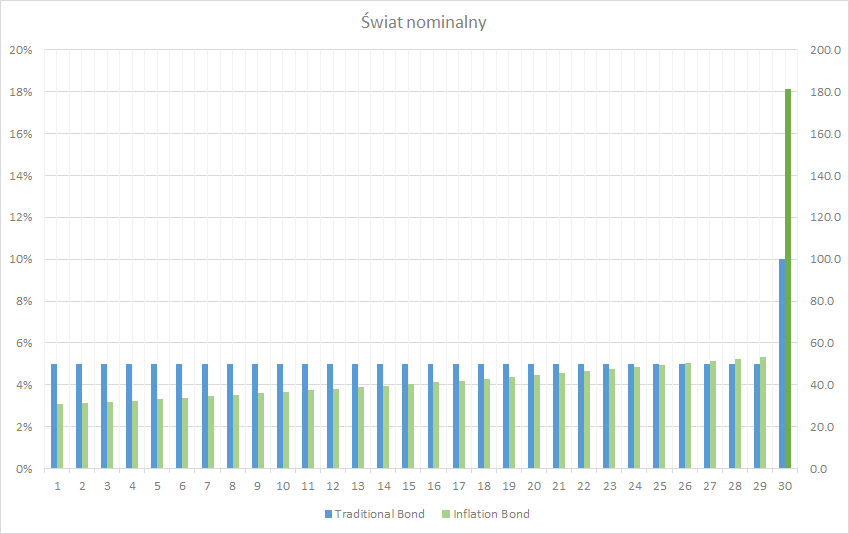
\includegraphics[scale=0.7]{graphics/nominalworld.png}
		\caption{Wykres przedstawiający przepływy w ramach porównania obligacji tradycyjnej i inflacyjnej udzielonych na 30 lat w ujęciu nominalnym.}
	\end{figure}
	W ujęciu rzeczywistym przepływy obu obligacji wyglądają zupełnie inaczej. Wartość rzeczywista przepływów obligacji indeksowanej do inflacji jest stała natomiast wartości nominalna (NV) 100 jednostek jest równa
		\begin{equation*}
	NV(t) = 100 * (1+2\%)^t.
	\end{equation*}
	Natomiast nominalna wartość jednego kuponu (NC) obligacji linkowanej do inflacji w chwili $t$ jest równa
	\begin{equation*}
	NC(t) = 3 * (1+2\%)^t.
	\end{equation*}
	\begin{figure} [h]
	\centering
	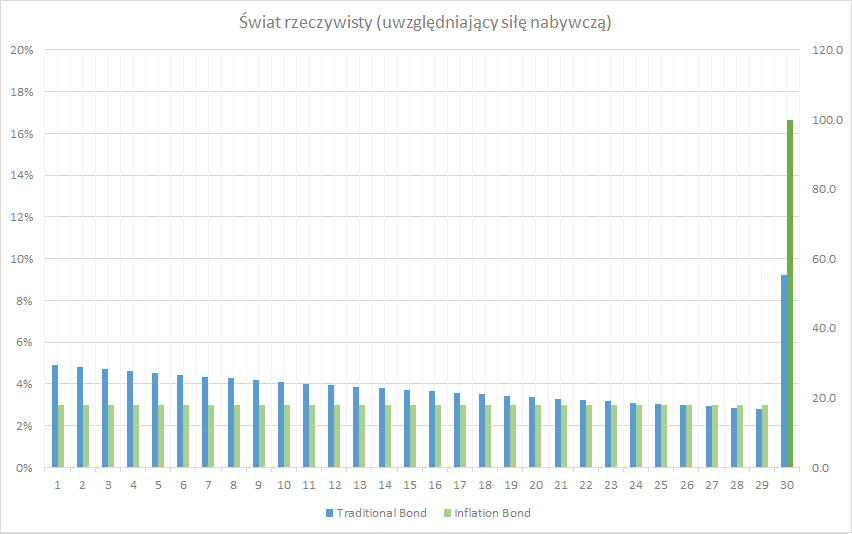
\includegraphics[scale=0.7]{graphics/realworld.png}
	\caption{Wykres przedstawiający przepływy w ramach porównania obligacji tradycyjnej i inflacyjnej udzielonych na 30 lat w ujęciu rzeczywistym.}
\end{figure}
	
\chapter{Modele rynkowe}

	W poniższym rozdziale wprowadzono i zaprezentowano jeden z najczęściej wykorzystywanych modeli do modelowania instrumentów powiązanych z inflacją. Wykorzystując analogię do modelowania walut obcych Jarrow and Yildirim zaproponowali model, w którym cena rzeczywista odpowiada procesowi cen w walucie obcej, cena nominalna procesowi cen w walucie krajowej natomiast indeks inflacyjny jest utożsamiany z kursem walutowym spot (ang. spot exchange rate). Rozważamy rynek zbudowany na bazie zwykłych obligacji zerokuponowych oraz tych indeksowanych do inflacji, bez ryzyka kredytowego. Celem modelowania jest ustalenie cen obligacji w taki sposób, aby otrzymać wolny od arbitrażu model rynku finansowego przy wykorzystaniu metody HJM modelowania struktury terminowej, a następnie wycena instrumentów pochodnych powiązanych z inflacją.
	
	\section{Model Jarrowa i Yildirima}
	
	\subsection*{Przestrzeń probabilistyczna}
		
	Rozważamy model rynku z czasem ciągłym na przedziale $[0,T^*]$, gdzie $T^* > 0$ jest ustalonym horyzontem czasowym. Będziemy rozważać obligację zerokuponową bez ryzyka kredytowego wypłacającą jedną jednostkę pieniędzy w ustalonej dacie wykupu $T \le T^*$. Poprzez indeks $n$ będziemy odnosić się do stopy nominalnej, zaś $r$ będzie oznaczać stopę rzeczywistą  - uwzględniające korektę wartością stopy inflacyjnej. Cenę nominalną obligacji w chwili $t \le T$ o terminie zapadalności $T \le T^*$  oznaczamy symbolem $P_n (t,T)$, natomiast cenę rzeczywistą obligacji zerokuponowej jako $P_r (t,T)$. Dodatkowo notowanie ustalonego indeksu zmiany cen w momencie $t$ będziemy oznaczać poprzez proces $I(t)$ dla każdego $t \le T$.\\
	\begin{Stwierdzenie}
		Niech $f_k(t,T)$ oznacza proces chwilowej stopy forward w momencie t dla $k \in \{n,r\}$ (odpowiednio względem stopy nominalnej i rzeczywistej). Dla dowolnego  $t \le T$ cena obligacji zerokuponowej o terminie zapadalności $T \le T^*$ jest równa
		\begin{eqnarray*}
			P_k(t,T) = \exp \bigg(-\int_t^T f_k(t,u) du \bigg).
		\end{eqnarray*}
	\end{Stwierdzenie}
	
	Dla każdego terminu wykupu $T$ warunek początkowy $f(0,T)$ jest określony przez bieżące wartości cen obligacji zerokuponowych. Standardowo wprowadzamy również dodatkowy dostępny instrument - rachunek oszczędnościowy. \\
	\begin{Stwierdzenie}
		Zakładamy, że istnieje mierzalna modyfikacja procesu chwilowej stopy forward $f(t,t)$ dla $t \le T^*$. Krótkoterminowa stopa procentowa spełnia warunek $r_k(t) = f_k(t,t)$ dla każdego t oraz dla $k \in \{n,r\}$. Proces rachunku oszczędnościowego jest równy
		\begin{eqnarray*}
			B_k(t) = \exp \bigg( \int_0^t f_k(u,u) du \bigg)
		\end{eqnarray*}
		dla każdego $t \in [0,T^*] $ oraz dla $k \in \{n,r\}$. 
	\end{Stwierdzenie}

	\subsection*{Trójczynnikowy model rynku}
	
	Rozważamy przestrzeń probabilistyczną  $(\Omega,\mathbb{F},\mathbb{P})$, gdzie $\mathbb{P}$ jest interpretowane jako prawdopodobieństwo rzeczywiste. Zakładamy, że filtracja $\mathbb{F} = (\mathcal{F}_t)_{t \in [0,T]}$ jest generowana przez trzy procesy Wienera:
	 \begin{eqnarray*}
		 W_n^{\mathbb{P}}(t), W_r^{\mathbb{P}}(t), W_I^{\mathbb{P}}(t).
	\end{eqnarray*}
	 gdzie $t \in [0,T^*]$. Procesy te startują w chwili $t = 0$ a korelacje pomiędzy nimi oznaczamy jako:
	\begin{align*}
		 dW_n^{\mathbb{P}}(t) dW_r^{\mathbb{P}}(t) &= \rho_{nr}dt, \\
		 dW_n^{\mathbb{P}}(t) dW_I^{\mathbb{P}}(t) &= \rho_{nI}dt, \\
		 dW_r^{\mathbb{P}}(t) dW_I^{\mathbb{P}}(t) &= \rho_{rI}dt.
	\end{align*}
	
	Rynek inflacji będziemy modelować za pomocą trzech czynników: nominalnej i rzeczywistej chwilowej stopy forward oraz procesu inflacji. Dla każdego z nich zostaną zdefiniowane odpowiednie równania dynamik.
	
	Dla dowolnego terminu wykupu $T \le T^*$ określamy warunek początkowy poprzez bieżące wartości nominalnych cen obligacji zerokuponowych $f_n^*(0,T)$. Dynamika nominalnej chwilowej stopy forward opisujemy jako:
	\begin{align*}
		df_n(t,T) &= \alpha_n(t,T)dt + \sigma_n(t,T) dW_n^{\mathbb{P}}(t),\\
		f_n(0,T)  &= f_n^*(0,T)
	\end{align*}
	gdzie procesy $\alpha_n$ oraz $\sigma_n$ są $\mathcal{F}$-adoptowanymi procesami stochastycznymi.
		
	Analogicznie przedstawiamy dla dowolnego terminu wykupu $T \le T^*$ dynamikę rzeczywistej chwilowej stopy forward:
	\begin{align*}
		df_r(t,T)  &= \alpha_r(t,T)dt + \sigma_r(t,T) dW_r^{\mathbb{P}}(t),\\
		 f_r(0,T) &= f_r^*(0,T)
	\end{align*}
	gdzie procesy $\alpha_r$ oraz $\sigma_r$ są $\mathcal{F}$-adoptowanymi procesami stochastycznymi oraz $f_r^*(0,T)$ jest krzywą terminową (rzeczywistą) bieżących cen obligacji zerokuponowych.  
	Ostatnim modelowanym czynnikiem jest indeks inflacyjny, dla którego zadajemy następującą postać dynamiki
	\begin{eqnarray*}
		\frac{dI(t)}{I(t)} = \mu_I(t)dt + \sigma_I(t)dW_I^{\mathbb{P}}(t),
	\end{eqnarray*}
	gdzie proces $\mu_I$ jest $\mathcal{F}$-adoptowanym procesem stochastycznym zaś $\sigma_I$ jest funkcją deterministycznym, co implikuje normalność rozkład logarytmu zmiennej losowej zmiany indeksu inflacji. Powyższe założenia pozwalają na zastosowanie podejścia HJM modelowania rynku obligacji.\\
	
	\begin{Twierdzenie}
		Trójczynnikowy model rynku Jarrowa and Yildirima jest pozbawiony arbitrażu i jest rynkiem zupełnym, jeżeli istnieje jedyna miara martyngałowa $\mathbb{Q}$ równoważna mierze ${\mathbb{P}}$ taka, że procesy:
		\begin{eqnarray*}
			\bigg(\frac{P_n(t,T)}{B_n(t)}\bigg)_{t\le T}, \bigg(\frac{I(t)P_r(t,T)}{B_n(t)}\bigg)_{t\le T}, \bigg(\frac{I(t)B_r(t)}{B_n(t)}\bigg)_{t\le T} 
		\end{eqnarray*}
		są \,$\mathbb{Q}$-martyngałami dla każdego $T \in [0,T^*]$.\\
	\end{Twierdzenie}	
	
	\begin{Uwaga}
		Ponadto korzystając z twierdzenia Girsanowa jeżeli procesy: $$(W_n(t))_{t\le T},(W_r(t))_{t\le T},(W_I(t))_{t\le T}$$ są procesami Wienera przy mierze rzeczywistej $\mathbb{P}$ oraz $\mathbb{Q}$ jest miarą probabilistyczną równoważną mierze $\mathbb{P}$, wówczas istnieją procesy premii za ryzyko:  $$(\lambda_n(t))_{t\le T},(\lambda_r(t))_{t\le T},(\lambda_I(t))_{t\le T}$$ takie, że
		\begin{eqnarray*}
			W^\mathbb{Q}_k(t) = W^\mathbb{P}_k(t) - \int_{0}^{t}\lambda_k(s)ds ,\,dla\, k\in\{n,r,I\}
		\end{eqnarray*}
		są procesami Wienera względem miary probabilistycznej $\mathbb{Q}$ dla każdego $t \in [0,T]$. 
	\end{Uwaga}
	
	Powyższe rozważania dotyczące struktury terminowej cen obligacji względem stopy nominalnej i rzeczywistej pozwalają na sformułowanie kluczowego twierdzenia przedstawiającego warunki konieczne i wystarczające do otrzymania rynku bez możliwości arbitrażu.\\
	
	\begin{Twierdzenie} \textbf{Bezarbitrażowa struktura terminowa}\\
		Zakładając, że dane są stopy forward prcesy:
		\begin{eqnarray*}
			\bigg(\frac{P_n(t,T)}{B_n(t)}\bigg)_{t\le T}, \bigg(\frac{I(t)P_r(t,T)}{B_n(t)}\bigg)_{t\le T}, \bigg(\frac{I(t)B_r(t)}{B_n(t)}\bigg)_{t\le T}
		\end{eqnarray*}
		są martyngałami względem miary martyngałowej $\mathbb{Q}$ wtedy i tylko wtedy, gdy:
		\begin{align}
		\alpha_n(t,T) &= \sigma_n(t,T)\bigg(\int_{t}^{T}\sigma_n(t,s)ds-\lambda_n(t)\bigg),\\
		\alpha_r(t,T) &= \sigma_r(t,T)\bigg(\int_{t}^{T}\sigma_r(t,s)ds-\sigma_I(t)\rho_{rl}-\lambda_r(t)\bigg),\\
		\mu_I(t) &= r_n(t)-r_r(t)-\sigma_I(t)\lambda_I(t).
		\end{align}
	\end{Twierdzenie}
	
	\begin{proof}
		
		Pierwsze równanie  jest warunkiem dryfu przy metodzie HJM dla nominalnej stopy forwardowej, analogicznie kolejne jest warunkiem dla rzeczywistej stopy forwardowej uwzględniające zmienność inflacji a także współczynnik korelacji pomiędzy inflacją a rzeczywistą stopą forwardową. Ostatnie równanie jest równaniem Fishera łączącym zależność pomiędzy nominalną i realną stopą procentową oraz oczekiwaną inflacją i premią za ryzyko inflacyjne. 

	\subsection*{Dynamika procesu cen obligacji}
	Punktem wyjścia do wyprowadzenia warunków koniecznych gwarantujących brak możliwości arbitrażu w trójfaktorowym modelu rynku inflacji jest postać dynamiki procesu cen obligacji zerokuponowej $P_k(t,T)$, gdzie $k \in\{r,n\}$. Określamy ją w następujący sposób
	\begin{equation*}
	dP_k(t,T) = P_k(t,T) \bigg((f(t,t)+\alpha_k^*(t,T)+\frac{1}{2} ||\sigma_k^*(t,T)||^2 )dt +\sigma_k^*(t,T) dW_k^\mathbb{P}(t)\bigg),
	\end{equation*}
	gdzie dla każdego $t\in[0,T]$ oznaczamy
	\begin{align}
	\alpha_k^*(t,T) &:= - \int_{t}^{T} \alpha_k(t,u) du,\\
	\sigma_k^*(t,T) &:= - \int_{t}^{T} \sigma_k(t,u) du.
	\end{align}
	\subsection*{Rachunek oszczędnościowy}
	Niech $B_r^*(t) = I(t) B_r(t)$. Otrzymujemy wówczas
	\begin{align*}
	d B_r^*(t) &= B_r(t) dI(t) + I(t)dB_r(t) \\
	&= B_r(t) dI(t) + I(t)r_r(t) B_r(t) dt \\
	&= B_r(t) (I(t) [\mu_I(t)dt + \sigma_I(t)dW_I^\mathbb{P}(t) ] + I(t)r_r(t)dt) \\
	&= B_r(t) I(t) ([\mu_I(t) + r_r(t) ]dt + \sigma_I(t) dW_I^\mathbb{P}(t)).
	\end{align*}
	Mamy więc
	\begin{equation}
	\frac{dB_r^*(t)}{B_r^*(t)} = [\mu_I(t) + r_r(t) ]dt + \sigma_I(t) dW_I^\mathbb{P}(t).
	\end{equation}
	Dynamika procesu $B_r^*(t)$ dyskontowanego procesem $B_n(t)$ zapiszemy jako
	\begin{align*}
	d\bigg(\frac{B_r^*(t)}{B_n(t)}\bigg) &= \frac{d B_r^*(t)}{B_n(t)} - \frac{B^*(t) d B_n(t)}{B_n(t)^2}\\
	&= \frac{d B_r^*(t)}{B_n(t)} - \frac{B_r^*(t)r_n(t)B_n(t)dt}{B_n(t)^2}\\
	&= \frac{d B_r^*(t)}{B_n(t)} - \frac{B_r^*(t)}{B_n(t)}r_n(t)\\
	&= \frac{B_r^*(t)}{B_n(t)} \bigg( [\mu_I(t) + r_r(t) - r_n(t)]dt + \sigma_I(t) dW_I^\mathbb{P}(t)\bigg).
	\end{align*}
	Względem miary martyngałowej $\mathbb{Q}$ równoważnej mierze $\mathbb{P}$:
	\begin{equation*}
	d\bigg(\frac{B_r^*(t)}{B_n(t)} \bigg) = \frac{B_r^*(t)}{B_n(t)} [\sigma_I(t) dW_I^\mathbb{P}(t)],
	\end{equation*}
	gdzie
	\begin{equation*}
	W_I^\mathbb{Q}(t) = W_I^\mathbb{P}(t) - \int_{0}^{t} \lambda_I(u) du.
	\end{equation*}
	Otrzymujemy wówczas warunek
	\begin{equation}
	\mu_I(t) + r_r(t) - r_n(t) = -\lambda_I(t) \sigma_I(t),
	\end{equation}
	i stąd
	\begin{equation}
	\mu_I(t) =  r_n(t) - r_r(t) - \lambda_I(t) \sigma_I(t).
	\end{equation}
	
	\subsection*{Struktura terminowa obligacji względem stopy nominalnej}
	Pierwszy proces bezarbitrażowej struktury terminowej
	\begin{align*}
	d\bigg(\frac{P_n(t,T)}{B_n(t)}\bigg)  &= \frac{dP_n(t,T)}{B_n(t)} - \frac{dB_n(t)P_n(t,T)}{B_n^2(t)}\\
	&= \frac{dP_n(t,T)}{B_n(t)} - \frac{B_n(t)r_n(t)dt P_n(t,T)}{B_n^2(t)} \\
	&= \frac{dP_n(t,T)}{B_n(t)} - \frac{P_n(t,T) r_n(t)dt }{B_n(t)} \\
	&=\frac{P_n(t,T)}{B_n(t)} \bigg[  \alpha_n^*(t,T) + \frac{1}{2} ||\sigma_n^*(t,T)||^2)dt + \sigma_n^*dW_n^\mathbb{P}(t)
	\end{align*}
	Otrzymujemy wówczas
	\begin{equation}
	\alpha_n^*(t,T) + \frac{1}{2} ||\sigma_n^*(t,T)||^2 = \lambda_n(t)\sigma_n^*(t,T)
	\end{equation}
	Różniczkując po T
	\begin{equation}
	-\alpha_n(t,T) + \sigma_n^*(t,T)\sigma_n(t,T) = \lambda_n(t)\sigma_n(t,T)
	\end{equation}
	Co prowadzi nas do
	\begin{align*}
	\alpha_n(t,T) &= - \lambda_n(t)\sigma_n(t,T) + \sigma_n^*(t,T)\sigma_n(t,T) \\
	\alpha_n(t,T) &= \sigma_n(t,T)\bigg[ -\lambda_n(t) + \int_{t}^{T}\sigma_n(t,u) du\bigg].
	\end{align*}
	Ostatecznie względem miary rzeczywistej $\mathbb{P}$ dynamikę obligacji względem stopy nominalnej możemy zapisać jako
	\begin{equation}
	\frac{dP_n(t,T)}{P_n(t,T)} = [r_n(t) +\sigma^*_n(t,T)\lambda_n(t)]dt + \sigma^*_r(t,T)dW^\mathbb{P}_n(t)
	\end{equation}
	zaś względem miary wolnej od ryzyka $\mathbb{Q}$ jako
	\begin{equation}
	\frac{dP_n(t,T)}{P_n(t,T)} = r_n(t)dt + \sigma^*_n(t,T)dW^\mathbb{Q}_n(t)
	\end{equation}
	
	\subsection*{Struktura terminowa obligacji względem stopy rzeczywistej}
	
	W analogiczny sposób jak wyżej oznaczamy strukturę terminową obligacji względem rzeczywistej stopy procentowej $P_r^*(t) = I(t) P_r(t, T)$. Dynamika procesu ceny obligacji jest równa
	\begin{equation}
	d P_r^*(t,T) = P_r(t,T) dI(t) + I(t)dP_r(t,T) + d<P_r(*,T), I(*)>_t.
	\end{equation}
	Przyjmując wcześniejsze oznaczenia nawias skośny jest równy
	\begin{equation*}
	d<P_r(*,T), I(*)>_t = I(t) \sigma_I(t) P_r(t,T)\sigma_r^*(t)\rho_{rI} dt.
	\end{equation*} 
	Podstawiając
	\begin{align*}
	d P_r^*(t,T) &= P_r(t,T) dI(t) + I(t)dP_r(t,T) + I(t) \sigma_I(t) P_r(t,T)\sigma_r^*(t)\rho_{rI} dt, \\
	&= I(t) P_r(t,T) \bigg(\bigg[ r_r(t) + \sigma^*_r(t,T) + \frac{1}{2} || \sigma^*(t,T) ||^2 + \mu_I(t) + \sigma_I(t)\sigma^*_r(t,T)\rho_{rI} \bigg] dt\\
	&+ \sigma^*(t)dW_r^\mathbb{P}(t) + \sigma_I(t) dW_I^\mathbb{P}(t) \bigg).
	\end{align*} 
	Stąd otrzymujemy
	\begin{equation*}
	\frac{dP_r^*(t,T)}{P_r^*(t,T)} = \bigg(\bigg[ r_r(t) + \sigma^*_r(t,T) + \frac{1}{2} || \sigma^*(t,T) ||^2 + \mu_I(t) + \sigma_I(t)\sigma^*_r(t,T)\rho_{rI} \bigg] dt + \sigma^*(t)dW_r^\mathbb{P}(t) + \sigma_I(t) dW_I^\mathbb{P}(t) \bigg).
	\end{equation*}
	Dynamika procesu $P_r^*(t,T)$ dyskontowanego procesem $B_n(t)$ jest równa
	\begin{align*}
	d\bigg(\frac{P^*_r(t,T)}{B_n(t)}\bigg) &= \frac{dP_r^*(t,T)}{B_n(t)} - \frac{dB_n(t)P_r^*(t,T)}{B_n^2(t)}\\
	&= \frac{dP_r^*(t,T)}{B_n(t)} - \frac{B_n(t)r_n(t)dt P_r^*(t,T)}{B_n^2(t)} \\
	&= \frac{dP_r^*(t,T)}{B_n(t)} - \frac{P_r^*(t,T)r_n(t)dt}{B_n^2(t)} \\
	&= \frac{P_r^*(t,T)}{B_n(t)} \bigg[ -r_n(t)dt + (r_r(t) + \alpha_r^*(t,T) + \frac{1}{2} ||\sigma_r^*(t,T)||^2 + \mu_I(t) + \sigma_I(t)\sigma_r^*(t,T)\rho_{rI})dt \\
	&+ \sigma^*_r(t,T)dW_r^\mathbb{P}(t) + \sigma_I(t)dW_I^\mathbb{P}(t) \bigg]\\
	&= \frac{P_r^*(t,T)}{B_n(t)} \bigg[ (-r_n(t) + r_r(t) + \alpha_r^*(t,T) + \frac{1}{2} ||\sigma_r^*(t,T)||^2 + \mu_I(t) + \sigma_I(t)\sigma_r^*(t,T)\rho_{rI})dt \\
	&+ \sigma^*_r(t,T)dW_r^\mathbb{P}(t) + \sigma_I(t)dW_I^\mathbb{P}(t) \bigg]
	\end{align*}
	Względem miary martyngałowej $\mathbb{Q}$ równoważnej mierze $\mathbb{P}$
	\begin{equation*}
	d\bigg(	\frac{P_r^*(t,T)}{B_n(t)}\bigg) = \frac{P_r^*(t,T)}{B_n(t)} [\sigma_r(t,T)dW_r^\mathbb{Q}(t) + \sigma_I(t,T)dW_I^\mathbb{Q}(t)],
	\end{equation*}
	gdzie
	\begin{align*}
	W_r^\mathbb{Q}(t) &= W_r^\mathbb{P}(t) - \int_{0}^{t} \lambda_r(u) du, \\
	W_I^\mathbb{Q}(t) &= W_I^\mathbb{P}(t) - \int_{0}^{t} \lambda_I(u) du.
	\end{align*}
	Otrzymujemy wówczas
	\begin{equation}
	-r_n(t) + r_r(t) + \alpha_r^*(t,T) + \frac{1}{2} ||\sigma_r^*(t,T)||^2 + \mu_I(t) + \sigma_I(t)\sigma_I(t,T).
	\end{equation}
	Różniczkując względem T
	\begin{equation}
	-\alpha_r(t,T) + \sigma_r^*(t,T)\sigma_r(t,T)-\sigma_I(t,T)\rho_{rI}\sigma_r(t,T) = \lambda_r(t)\sigma_r(t,T)
	\end{equation}
	Prowadzi nas to warunku dryfu względem stopy rzeczywistej
	\begin{align*}
	\alpha_r(t,T) &= \lambda_r(t)\sigma_r(t,T) + \sigma_r^*(t,T)\sigma_r(t,T)+\sigma_I(t,T)\rho_{rI}\sigma_r(t,T) \\
	\alpha_r(t,T) &= \sigma_r(t,T)\bigg[ -\lambda_r(t) + \int_{t}^{T}\sigma_r(t,u) du - \sigma_I(t,T)\rho_{rI}\bigg].
	\end{align*}
	Ostatecznie względem miary rzeczywistej P dynamikę obligacji względem stopy rzeczywistej możemy zapisać jako
	\begin{equation}
	\frac{dP_r(t,T)}{P_r(t,T)} = [r_r(t) +\sigma^*_r(t,T)(\sigma_I(t,T)\rho_{rI}-\lambda_r(t))]dt + \sigma^*_r(t,T)dW^\mathbb{P}_r.
	\end{equation}
	Zaś względem miary wolnej od ryzyka Q jako
	\begin{equation}
	\frac{dP_r(t,T)}{P_r(t,T)} = [r_r(t) +\sigma^*_r(t,T)\sigma_I(t,T)\rho_{rI}]dt + \sigma^*_r(t,T)dW^\mathbb{Q}_r.
	\end{equation}

		\end{proof}

	\begin{Twierdzenie} \textbf{Procesy cen względem miary martyngałowej spot}\\
	Względem miary martyngałowej spot zachodzą następujące równości
		\begin{align}
		df_n(t,T) &= -\sigma_n(t,T) \sigma^*_n(t,T)dt + \sigma_n(t,T)dW_n^\mathbb{Q}(t) \\
		df_r(t,T) &= -\sigma_r(t,T) [\sigma^*_r(t,T) + \rho_{rI}\sigma_I(t)]dt + \sigma_r(t,T)dW_r^\mathbb{Q}(t)\\
		\frac{dI(t)}{I(t)} &= [r_n(t) - r_r(t)] dt + \sigma_I(t)dW_I^\mathbb{Q}(t)\\
		\frac{dP_n(t,T)}{P_n(t,T)} &= r_n(t)dt + \sigma^*_n(t,T)dW_n^\mathbb{Q}(t)\\
		\frac{dP_r(t,T)}{P_r(t,T)} &= [r_r(t) - \sigma^*_r(t,T)\sigma_I(t)\rho_{rI}]dt + \sigma^*_r(t,T) dW_r^\mathbb{Q}(t)\\
		\frac{dP_{IL}(t,T)}{P_{IL}(t,T)} &:= \frac{d(I(t)P_r(t,T))}{I(t)P_r(t,T)} = r_n(t)dt + \sigma_I(t)dW_I^Q(t) + \sigma^*_r(t,T) dW_r^\mathbb{Q}(t).  
		\end{align}
	\end{Twierdzenie}

\begin{proof}
	 Dowód powyższych równości jest naturalną kontynuacją rozważań w dowodzie dla warunków koniecznych i wystarczających bezarbitrażowej struktury terminowej polegającym na zamianę miary na wolną ryzyka.
	 
	 W strukturze terminowa obligacji względem stopy nominalnej otrzymaliśmy dynamikę względem stopy nominalnej przy mierze rzeczywistej $\mathbb{P}$
	 \begin{equation}
	 \frac{dP_n(t,T)}{P_n(t,T)} = [r_n(t) +\sigma^*_n(t,T)\lambda_n(t)]dt + \sigma^*_r(t,T)dW^\mathbb{P}_n(t)
	 \end{equation}
	 Względem miary wolnej od ryzyka Q otrzymujemy
	 \begin{equation}
	 \frac{dP_n(t,T)}{P_n(t,T)} = r_n(t)dt + \sigma^*_n(t,T)dW^\mathbb{Q}_n(t).
	 \end{equation}
	 Z kolei dla struktury terminowej obligacji względem stopy realnej dynamika obligacji przy stopie rzeczywistej względem miary rzeczywistej P jest równa
	 \begin{equation}
	 \frac{dP_r(t,T)}{P_r(t,T)} = [r_r(t) +\sigma^*_r(t,T)(\sigma_I(t,T)\rho_{rI}-\lambda_r(t))]dt + \sigma^*_r(t,T)dW^\mathbb{P}_r,
	 \end{equation}
	 zaś względem miary wolnej od ryzyka Q otrzymujemy
	 \begin{equation}
	 \frac{dP_r(t,T)}{P_r(t,T)} = [r_r(t) +\sigma^*_r(t,T)\sigma_I(t,T)\rho_{rI}]dt + \sigma^*_r(t,T)dW^\mathbb{Q}_r.
	 \end{equation}
	 
	 
\end{proof}
	
	\section{Uogólniony model Vasicka}
	Jednym z pierwszych modeli stopy krótkoterminowej jest model zaproponowany przez Vasi\v{c}ka w roku 1977, w którym dynamika stopy $r$ w mierze $\mathbb{P}^*$ jest zadana przez równanie
	\begin{equation}
	 dr_t =(\theta -ar_t)dt+\sigma dW_t^*
	\end{equation}
	dla stałych $r_0,\theta,a,\sigma >0$. Stopa krótkoterminowa w tym modelu ma tzw. \textit{własność powrotu do średniej}: w przypadku, gdy $r_t < \frac{\theta}{a}$, dryf procesu jest dodatni; jeśli zaś $r_t > \frac{\theta}{a}$, to dryf jest ujemny. Zatem dla każdego $t$ stopa krótkoterminowa $r_t$ zbiega do wartości $\frac{\theta}{a}$. 
	
	Wadą modelu Vasi\v{c}ka jest brak dokładnej możliwości dopasowania go do bieżącej struktury terminowej stóp procentowych. Aby dokładnie skalibrować model do rynkowych cen obligacji, musielibyśmy rozwiązać nieskończoną liczbę równań postaci
	\begin{equation}
	B(0,T) = \mathbb{E}_{\mathbb{P}^*}
	\left(\exp\bigg(-\int_0^T r_sds\bigg)\right), \quad T \in [0,T^*], 
	\end{equation}
	co wymagałoby wprowadzenia nieskończenie wielu parametrów. Ten problem stanowił motywację dla Hulla i White'a do rozszerzenia modelu Vasi\v{c}ka poprzez zastąpienie stałych parametrów funkcjami zależnymi od czasu i modelowanie stopy krótkoterminowej równaniem
	\begin{equation}
	dr_t =(\theta(t) -a(t)r_t)dt+\sigma(t) dW_t^*, \quad r_0,
	\end{equation}
	gdzie funkcje $\theta,a,\sigma: [0,T^*] \to \mathbf{R}$ są ograniczone. \textit{Uogólniony model Vasi\v{c}ka}, daje możliwość dokładnej kalibracji do początkowej struktury terminowej stóp procentowych. Ponadto zachowuje on własność powrotu do średniej w tym sensie, że dla każdego $t$ stopa krótkoterminowa $r_t$ zbliża się do krzywej $\frac{\theta(t)}{a(t)}$ ($a(t) \neq 0$). Parametr $a(t)$ bywa nazywany \textit{parametrem powrotu do średniej}.
	\subsection{Rzeczywista i nominalna struktura terminowa w uogólnionym modelu Vasicka}
	Jarrow i Yildirim do modelowania stopy krótkoterminowej zarówno w podejściu nominalnym jak i realnym proponują zastosowanie uogólnionego modelu Vasicka. \\
	\begin{Lemat}
		Niech proces stopy krótkoterminowej $r_k$, gdzie $k \in \{n, r\}$ spełnia równie
		\begin{equation}
		dr_k(t) = (a_k(t) - b_k(t)r_k(t))dt + \sigma_k(t)dW^*_k(t),
		\end{equation}
		gdzie $W^*$ jest jednowymiarowym procesem Wienera zaś $a_k, b_k, \sigma_k$ są lokalnie ograniczonymi funkcjami. Ponadto zakładamy, że funkcja zmienności przyjmuje następującą postać
		\begin{equation}
		\sigma_k(t,T) = \sigma_k e^{-\kappa_k (T-t)}.
		\end{equation}
		Ponadto niech
		\begin{equation}
		a_k(t,T) = - \int_t^T \sigma_k(t,u) du = -\sigma_k \int_t^T e^{-\kappa_k(u-t)}du = -\sigma_k\beta_k(t,T),
		\end{equation}
		gdzie 
		\begin{equation}
		\beta_k(t,T) = \frac{1}{\kappa_k} [1 - e^{-\kappa_k(T-t)}].
		\end{equation}
		Wówczas nominalną i rzeczywista struktura terminowa jest równa
		\begin{align}
		P_n(t, T) &= \frac{P_n(0,T)}{P_n(0,T)} \exp\bigg( \beta_n (t, T) [f_n(0,t) - r_n(t) ]  - \frac{\sigma_n^2}{4\kappa_n} \beta_n^2(t,T) [1 - e^{-2\kappa_n t}] \bigg),\\
		P_r(t, T) &= \frac{P_r(0,T)}{P_r(0,T)} \exp\bigg( \beta_r (t, T) [f_r(0,t) - r_r(t) ]  - \frac{\sigma_r^2}{4\kappa_r} \beta_r^2(t,T) [1 - e^{-2\kappa_rt}] \bigg).
		\end{align}
	\end{Lemat}
	\begin{proof}
	Przy mierze martyngałowej $Q$ równanie stopy forward dla $k \in \{n, r\}$ przyjmuje postać
	\begin{equation}
		f_k(t,T) = f_k(0,T) + \sigma_k^2 \int_0^t \beta_k(s,T)e^{-\kappa_k(T-s)}ds + \sigma_k \int_0^t e^{-\kappa_k(T-s)}dW_k^\mathbb{Q}(s).
	\end{equation}
	Natomiast dla stopy krótkoterminowej $r_k = f_k(t, t)$ otrzymujemy
	\begin{align*}
		r_k(t) &= f_k(0,t) + \sigma_k^2 \int_0,t \beta_k(s,t) e^{-\kappa_k(T-s)}ds + \sigma_k \int_0^t e^{-\kappa_k(T-s)}dW_k^\mathbb{Q}(s)\\
		&= f_k(0,t) + \frac{\sigma_k^2}{2} \int_0^t \frac{\delta\beta_k^2(s,t)}{\delta t}ds + \sigma_k\int_0^t e^{-\kappa_k(T-s)}dW_k^Q(s)\\
		&= f_k(0,t) + \frac{\sigma_k^2}{2}\frac{\delta}{\delta t} \bigg(\int_0^t\beta_k^2(s, t)ds\bigg) + \sigma_k\int_0^t e^{-\kappa_k(T-s)}dW_k^\mathbb{Q}(s)
	\end{align*}
	Całkując stopę krótkoterminową dostajemy
	\begin{equation}
		\int_{0}^{t} r_k(u) du = ln P_k(0,t) + \frac{\sigma_k^2}{2} \int_{0}^{t} \beta^2_k(s,t) ds + \int_{0}^{t}\bigg[ \sigma_k \int_{0}^{t} e^{-\kappa_k(u-s)}dW_k^\mathbb{Q}(s)\bigg] du
	\end{equation}
	Wprowadzając proces $Y(t) = \int_{0}^{t}e^{as}dW_k^\mathbb{Q}(s)$ możemy zapisać
	\begin{align}
		d(e^{-at}Y(t)) &= e^{-at}dY(t) - ae^{-at}Y(t)dt \\
		&= dW_k^Q(t) - ae^{at}T(t)dt.
	\end{align}
	Całkując dostajemy
	\begin{equation}
		e^{-at}Y(t) = W_k^Q(t) - \int_{0}^{t} ae^{-au}Y(u) du.
	\end{equation}
	Wracając do całkowania procesu stopy krótkoterminowej rozpisujemy część wyrażenia zawierającego podwójne całkowanie
	\begin{align*}
		a\int_{0}^{t} \bigg[ e^{-au} \int_{0}^{u} e^{as}dW_k^Q(s) \bigg]du &= W_k^Q(t) - e^{-at}\int_{0}^{t} e^{au} dW_k^\mathbb{Q}(u) \\
		&= \int_{0}^{t} \bigg( 1 - e^{-a(t-u)}\bigg) dW_k^\mathbb{Q}(u) \\
		&= a \int_{0}^{t} \beta(u,t)dW_k^\mathbb{Q}(u).
	\end{align*}
	Wobec powyższego całkę procesu stopy krótkoterminowej zapiszemy jako
	\begin{equation}
		\int_{0}^{t} r_k(u) du = -\ln P_n(0,t) + \ln P_k(0,t) + \frac{\sigma_k^2}{2} \int_{0}^{t} \beta^2_k(s,t) ds + \sigma_k \int_{0}^{t} \beta_k(s,t) dW_k^\mathbb{Q}(s).
	\end{equation}
	Podstawiając wyprowadzany wzór do ceny obligacji zerokuponowej otrzymujemy
	\begin{align}
		P_k(t,T) &= P_k(0,T) \exp\bigg[ \int_{0}^{t}\bigg( r_k(t) - \frac{\sigma_k^2}{2}\beta_k^2(s,T)\bigg)ds - \sigma_k\int_{0}^{t} \beta_k(s,T)dW_k^\mathbb{Q}(s)  \bigg] \\
		&= \frac{P_k(0,T)}{P_k(0,t)} \exp \bigg[ \frac{\sigma_k^2}{2} \int_{0}^{t} (\beta_k^2(s,t) - \beta_k^2(s,T))ds + \sigma_k\int_{0}^{t} (\beta_k(s,t) - \beta_k(s,T)) dW_k^\mathbb{Q}(s) \bigg]
	\end{align}
	Zajmiemy się teraz wyrażeniem wewnątrz funkcji $\exp$. Oznaczmy
	\begin{equation}
		\delta = \bigg[ \frac{\sigma_k^2}{2} \int_{0}^{t} (\beta_k^2(s,t) - \beta_k^2(s,T))ds + \sigma_k\int_{0}^{t} (\beta_k(s,t) - \beta_k(s,T)) dW_k^Q(s) \bigg]
	\end{equation}
	Wartość $-\beta_k(t,T)r_k(t)$ jest równa
	\begin{align}
		-\beta_k(t,T)r_k(t) &= -\beta_k(t,T)f_k(0,t) + \sigma_k^2\int_{0}^{t} [\beta_k^2(s,t) - \beta_k(s,T)\beta_k(s,t)]ds \\ &+ \sigma_k\int_{0}^{t} [\beta_k(s,t) - \beta_k(s,T)]dW_k^\mathbb{Q}(s).
	\end{align}
	Wracając do wyrażenia powyżej
	\begin{align}
		\delta &= \beta_k(t,T)[f_k(0,t) - r_k(t)]-\frac{\sigma_k^2}{2}\int_{0}^{t}[\beta_k(s,t) + \beta_k(s,T)]^2ds \\
		&= \beta_k(t,T)[f_k(0,t) - r_k(t)]-\frac{\sigma_k^2}{4\kappa_k}\beta_k^2(t,T)[1-e^{-2\kappa_kt}] 
	\end{align}
	Stąd dostajemy wzory na nominalną i rzeczywistą strukturę terminową
	\begin{align}
		P_n(t, T) &= \frac{P_n(0,T)}{P_n(0,T)} \exp\bigg( \beta_n (t, T) [f_n(0,t) - r_n(t) ]  - \frac{\sigma_n^2}{4\kappa_n} \beta_n^2(t,T) [1 - e^{-2\kappa_n t}] \bigg),\\
		P_r(t, T) &= \frac{P_r(0,T)}{P_r(0,T)} \exp\bigg( \beta_r (t, T) [f_r(0,t) - r_r(t) ]  - \frac{\sigma_r^2}{4\kappa_r} \beta_r^2(t,T) [1 - e^{-2\kappa_rt}] \bigg).
	\end{align}
\end{proof}
	
	
	
	\pagebreak
\section{Przegląd pozostałych podejść do modelowania inflacji}
\subsection{Modele rynku Mercuria}
W 2004r. Mercurio przedstawił dwa modele rynkowe do modelowania instrumentów pochodnych indeksowanych do inflacji.  Pierwsze z nich opiera się na  podejściu do modelowania z zastosowaniem rynkowego modelu lognormalnego LIBOR do modelowania stóp procentowych zarówno dla krzywych nominalnych jak i rzeczywistych oraz indeksu inflacji procesem Wienera jak w przypadku modelu Jarrowa i Yildirima. Drugi model zaproponowany przez Merciuria wykorzystuje założenie, że stawki forwardowe indeksu inflacji są martyngałem w pewnym określonym okresie czasu.



\subsection{Model Beldgrade-Benhamou-Koehlar Market}	
Model zaproponowany przez Belgrade, Benhamou i Koehler jest modelem rynkowym i opiera się na wykorzystaniu kwotowań instrumentów o dużej płynności. Podejście zakłada brak arbitrażu pomiędzy stawkami zerokuponowymi oraz Year-on-Year kontraktów swapowych. Dodatkowym założeniem jest niewielka ilość parametrów oraz replikowanie cen rynkowych. Stawki forward indeksu inflacji są modelowane stochastycznie ze zmienność zadaną deterministycznie. Rozważano dwa przypadku podejścia do zmienności: model Blacka Scholesa oraz Hulla White. W pierwszym z nich, gdzie zmienność jest zadana przez funkcję deterministyczną i jednorodną wyprowadzono wzór dla zmienności Year-on-Year jako funkcji zmienności zerokuponowej.



	\chapter{Wycena w modelu Jarrowa i Yieldirima}
	
	W poniższym rozdziale zostały omówione i wyprowadzone wzory na wyceny w modelu Jarrowa i Yieldirima dla podstawowych instrumentów indeksowanych do inflacji: swapa zerokuponowego, swapa Year-on-Year oraz opcji inflacyjnych.
		
	\section{Wycena zerokuponowego swapa indeksowanego do inflacji}
	
	\begin{Lemat}
		Oznaczmy przez $\textbf{ZCIIS}(t,T_M,I_0,N)$ proces wartości zerokuponowego swapa indeksowanego do inflacji o terminie zapadalności $T_M$, nominale $N$ i początkowej wartości indeksu referencyjnego inflacji $I_0$. Wówczas cena takiego kontraktu w chwili $t$ jest równa
		\begin{eqnarray}
			\textbf{ZCIIS} (t,T_M,I_0,N) = N \bigg[\frac{I(t)}{I_0} P_r(t,T_M) - P_n(t,T_M)\bigg].
		\end{eqnarray}
		W szczególności cena w chwili 0 jest równa
		\begin{eqnarray}
			\textbf{ZCIIS} (0,T_M,I_0,N) = N [P_r(0,T_M) - P_n(0,T_M)].
		\end{eqnarray}
	\end{Lemat}
	\begin{proof}
	Korzystając z standardowej teorii wyceny bez arbitrażu w chwili t, dla czasu zapadalności $T_M$, przy wybranym indeksie referencyjnym $I_0$ i nominale kontraktu $N$ otrzymujemy
	\begin{eqnarray}
		\textbf{ZCIIS} (t,T_M,I_0,N) = N \mathbb{E}^{Qn} \bigg[e^{-\int_t^{T_M}r_n(u)du}\bigg(\frac{I(T_M)}{I_0}-1\bigg) \bigg| \mathcal{F}_t\bigg].
	\end{eqnarray}
	Korzystając z zamiany num\'{e}raire dochodzimy do równości
	\begin{eqnarray*}
		I(t) P_r (t,T_M) = I(t) \mathbb{E}^{Qr} \bigg[e^{-\int_t^{T_M}r_r(u)du} \bigg| F_t\bigg] = I(t) \mathbb{E}^{Qn} I(t_M) \bigg[e^{-\int_t^{T_M}r_n(u)du}\bigg(\frac{I(T_M)}{I_0}-1\bigg) \bigg| \mathcal{F}_t\bigg].
	\end{eqnarray*}
	Skąd otrzymujemy wzór na cenę zerokuponowego swapa indeksowanego do inflacji
	\begin{eqnarray}
		\textbf{ZCIIS} (t,T_M,I_0,N) = N \bigg[\frac{I(t)}{I_0} P_r(t,T_M) - P_n(t,T_M)\bigg].
	\end{eqnarray}
	W szczególności w momencie $t = 0$ dostajemy
	\begin{eqnarray}
		\textbf{ZCIIS} (0,T_M,I_0,N) = N [P_r(0,T_M) - P_n(0,T_M)]]
	\end{eqnarray}
	\end{proof}
	Ceny te nie zależą od żadnych założeń dynamik stóp procentowych i wynikają z braku arbitrażu na rynku. Dzięki temu krzywą realnej stopy dyskontowej możemy skalibrować do cen indeksowanych inflacją swapów zerokuponowych. \\
	\begin{Lemat}
		Niech $b(0,T_M)$ oznacza stopę rentowności kwotowaną na rynku dla terminu zapadalności $T_M$. Wówczas zależność między rzeczywistą $P_r(0,T_M)$ oraz nominalną $P_n(0,T_M)$ krzywą dyskontową opisuje równość
		\begin{eqnarray}
		P_r(0,T_M) = P_n(0,T_M)[1 + b(0,T_M)]^{T_M}.
		\end{eqnarray}
	\end{Lemat}
	\begin{proof}
		Wchodząc w kontrakt swapowy wartość obu nóg jest w chwili początkowej $t = 0$ są równe. Otrzymujemy więc
		\begin{eqnarray*}
			N P_n(0,T_M)[(1 + b(0,T_M))^{T_M} - 1] = N [P_r(0,T_M) - P_n(0,T_M)]].
		\end{eqnarray*}
		A stąd zależność pomiędzy rzeczywistą i nominalną krzywą dyskontową możemy zapisać jako
		\begin{eqnarray}
		P_r(0,T_M) = P_n(0,T_M)[1 + b(0,T_M)]^{T_M}.
		\end{eqnarray}
		gdzie $b(0,T_M)$ oznacza stopę rentowności kwotowaną na rynku.
	\end{proof}

	\section{Wycena swapa Year-on-Year indeksowanego do inflacji}
		
	\begin{Lemat}
			Oznaczmy przez $\textbf{YYIIS}(t,T_{i-1},T_{i},\psi_i,N)$ proces wartości przepływu swapa Year-on-Year indeksowanego do inflacji w okresie od $(T_{i-1}, T_i)$, nominale $N$ i frakcji roku $\psi_i$. Wówczas wartość przepływu w chwili $t$ jest równa
			\begin{eqnarray}
			\textbf{YYIIS} (t,T_{i-1},T_i,\psi_i,N) = N \psi_i \mathbb{E}^{\mathbb{Q}_n} \bigg[ e^{-\int_t^{T_i}r_n(u)du} P_r(T_{i-1},T_i) \bigg| \mathcal{F}_t \bigg] - N \psi_i P_n(t,T_i). 
			\end{eqnarray}
	\end{Lemat}
	\begin{proof}
		Korzystając z uprzednio przedstawionej formuły wyceny dla instrumentów zerokuponowych cena pojedynczej nogi kontraktu Year-on-Year jest równa
		\begin{eqnarray}
			\textbf{YYIIS} (t,T_{i-1},T_i,\psi_i,N) = N \psi_i \mathbb{E}^{\mathbb{Q}_n} \bigg[e^{-\int_t^{T_i}r_n(u)du}\bigg(\frac{I(T_i)}{I(T_{i-1})}-1\bigg) \bigg| \mathcal{F}_t\bigg].
		\end{eqnarray}
		Jeśli $t > T_{i-1}$ wartość $I(T_{i-1})$ jest znana. W takim przypadku wycena kontraktu YYIIS sprowadza do wyceny ZCIIS. W przeciwnym wypadku, jeżeli $t < T_{i-1}$ otrzymujemy
		\begin{align*}
		\textbf{YYIIS} (t,T_{i-1},T_i,\psi_i,N) &= N \psi_i \mathbb{E}^{\mathbb{Q}_n} \bigg[ \mathbb{E}^{\mathbb{Q}_n} \bigg[e^{-\int_t^{T_i}r_n(u)du}\bigg(\frac{I(T_i)}{I(T_{i-1})}-1\bigg) \bigg| F_{T_{i-1}}\bigg] \bigg| \mathcal{F}_t \bigg]\\
		&= N \psi_i \mathbb{E}^{\mathbb{Q}_n} \bigg[ e^{-\int_t^{T_{i-1}}r_n(u)du} \mathbb{E}^{\mathbb{Q}_n} \bigg[e^{-\int_{T_{i-1}}^{T_i}r_n(u)du}\bigg(\frac{I(T_i)}{I(T_{i-1})}-1\bigg) \bigg| \mathcal{F}_{T_{i-1}}\bigg] \bigg| \mathcal{F}_t \bigg].
		\end{align*}
		Przy czym prawda jest
		\begin{eqnarray*}
			\mathbb{E}^{\mathbb{Q}_n} \bigg[e^{-\int_{T_{i-1}}^{T_i}r_n(u)du}\bigg(\frac{I(T_i)}{I(T_{i-1})}-1\bigg) \bigg| \mathcal{F}_{T_{i-1}}\bigg] = \textbf{ZCIIS} (T_{i-1},T_I,i(t_{I-1}),1).
		\end{eqnarray*}
		Stąd po podstawieniu wartości wyznaczonej w poprzednim rozdziale otrzymujemy
		\begin{align*}
		\textbf{YYIIS} (t,T_{i-1},T_i,\psi_i,N) &= N \psi_i \mathbb{E}^{\mathbb{Q}_n} \bigg[ e^{-\int_t^{T_i}r_n(u)du} [P_r(T_{i-1},T_i) - P_n(T_{i-1,Ti})] \bigg| \mathcal{F}_t \bigg]\\
		&= N \psi_i E^{\mathbb{Q}_n} \bigg[ e^{-\int_t^{T_i}r_n(u)du} P_r(T_{i-1},T_i) \bigg| \mathcal{F}_t \bigg] - N \psi_i P_n(t,T_i). 
		\end{align*}
	\end{proof}
\begin{Uwaga}
		Wyrażanie 
			\begin{equation*}
		\mathbb{E}^{Qn} \bigg[ e^{-\int_t^{T_i}r_n(u)du} P_r(T_{i-1},T_i) \bigg| \mathcal{F}_t \bigg],
		\end{equation*}
		możemy interpretować jako cenę nominalną instrumentu wypłacającego w chwili $T_{i-1}$ (w jednostkach nominalnych) realną cenę obligacji zerokuponowej o dacie zapadalności $T_i$. Zakładając, że stopa rzeczywista jest deterministyczna dostajemy
	\begin{align}
	\mathbb{E}^{\mathbb{Q}_n} \bigg[ e^{-\int_t^{T_i}r_n(u)du} P_r(T_{i-1},T_i) \bigg| \mathcal{F}_t \bigg] &= P_n(t,T_{i-1})P_r(T_{i-1},T_i)\\
	&= P_n(t,T_{i-1})\frac{P_r(t,T_i)}{P_r(t,T_{i-1})}.
		\end{align}	
\end{Uwaga}
	W praktyce jednak założenie, że stopy rzeczywiste są deterministyczne jest nierealistyczne, więc wyprowadzony wcześniej wzór na cenę instrumentu Year-on-Year jest zależny od modelu.

	\section{Wycena swapa Year-on-Year Inflation Swap w modelu Jarrowa i Yieldirima}
	\begin{Lemat}
		Wartość $\textbf{YYIIS}(t,T_{i-1},T_{i},\psi_i,N)$ procesu pojedynczego przepływu swapa Year-on-Year indeksowanego do inflacji w okresie $(T_{i-1}, T_i)$, nominale $N$ i frakcji roku $\psi_i$ w modelu Jarrowa i Yieldirima w chwili $t$ jest równa
		\begin{equation*}
		\textbf{YYIIS}(t, T_{i-1},T_i,\psi_i,N) = N \psi_i \bigg[ P_n(t,T_{i-1}) \frac{P_r(t,T_2)}{P_r(t,T_1)} e^{C(t,T_1,T_2)} - P_n(t,T_i) \bigg],
		\end{equation*}
		gdzie
		\begin{align*}
		C(t,T_{i-1},T_i) &= \sigma_r\beta_r(T_{i-1},T_i) \bigg[ \beta_r(t,T_{i-1}) \bigg( \rho_{rI}\sigma_I - \frac{1}{2} \beta_r (t,T_{i-1}) 
		+ \frac{\rho_{nr}\sigma_n}{\kappa_r + \kappa_n} (1+a_r\beta_n(t,T_{i-1})) \bigg)\\&-  \frac{\rho_{nr}\sigma_n}{\kappa_r + \kappa_n} \beta_n(t,T_{i-1}) \bigg].
		\end{align*}
	\end{Lemat}
	\begin{proof}
	Z poprzedniej sekcji wiemy, że
	\begin{equation*}
	\textbf{YYIIS}(t,T_{i-1},T_i,\psi_i,N) = N\psi_i (P_n(t,T_{i-1})\mathbb{E}^{T_{i-1}}[P_r(T_{i-1},T_i)|F_t]-P_n(t,T_i)).
	\end{equation*}
	Dynamika procesu $P_r(t,T_2)$ przy mierze martyngałowej $T_1-forward$ możemy zapisać jako
	\begin{align*}
	P_r(t, T_2) &= P_r(0, T_2) \exp \bigg( \int_{0}^{t} (r_r(s) - a_r(s, T_2) \sigma_I(s)\rho_{rI} + a_r(s, T_2)a_n(s, T_1)\rho_{nr}) ds \bigg) \\
	&* \exp \bigg(-\int_{0}^{t} \frac{a^2_r(s, T_2)}{2}ds + \int_{0}^{t} a_r(s, T_2)dW_r^{T_1}(s)\bigg).
	\end{align*}
	Korzystając z eksponenty stochastycznej
	\begin{equation*}
		\mathcal{E} (X(t)) = exp \bigg(X(t) - \frac{1}{2}<X,X>_t\bigg).
	\end{equation*}
otrzymujemy
	\begin{align*}
	\frac{P_r(t,T_2)}{P_r(t,T_1)} &= \frac{P_r(0,T_2)}{P_r(0,T_1)} \mathcal{E}  \bigg( \int_{0}^{t} [a_r(s,T_2) - a_r(s,T_1)]dW_r^{T_1}(s)\bigg)\\
	&*exp\bigg(\int_{0}^{t} [a_r(s,T_2) - a_r(s,T_1)][a_n(s,T_1)\rho_{nr} - \sigma_I(s)\rho_{rI} - a_r(s,T_1)]ds \bigg)
	\end{align*}
	Przyjmując $t = T_1$ mamy
	\begin{align*}
	P_r(T_1,T_2) &= \frac{P_r(0,T_2)}{P_r(0,T_1)} \mathcal{E} \bigg( \int_{0}^{T_1} [a_r(s,T_2) - a_r(s,T_1)]dW_r^{T_1}(s)\bigg)\\
	&*exp\bigg(\int_{0}^{T_1} [a_r(s,T_2) - a_r(s,T_1)][a_n(s,T_1)\rho_{nr} - \sigma_I(s)\rho_{rI} - a_r(s,T_1)]ds \bigg)
	\end{align*}
	Co jest równoważne
	\begin{equation*}
	P_r(T_1,T_2) | \mathcal{F}_t = \frac{P_r(t,T_2)}{P_r(t,T_1)} \mathcal{E}  \bigg( \int_{0}^{T_1} [a_r(s,T_2) - a_r(s,T_1)]dW_r^{T_1}(s)\bigg) * e^{C(t,T_1,T_2)}
	\end{equation*}
	gdzie
	\begin{equation*}
	C(t,T_1,T_2) = \int_{0}^{T_1} [a_r(s,T_2) - a_r(s,T_1)][a_n(s,T_1)\rho_{nr} - \sigma_I(s)\rho_{rI} - a_r(s,T_1)]ds.
	\end{equation*}
	Stąd
	\begin{equation*}
	\mathbb{E}^{T_1}[P_r(T_1,T_2) | \mathcal{F}_t] = \frac{P_r(t,T_2)}{P_r(t,T_1)} e^{C(t,T_1,T_2)}
	\end{equation*}
	Oczekiwana przyszła cena rzeczywista obligacji zerokuponowej względem miary forwardowej jest równa obecnej realnej cenie forwardowej pomnożonej przez czynnik korygujący. Czynnik ten zależy od zmienności i korelacji stopy nominalnej, rzeczywistej i indeksu inflacyjnego. Podstawiając otrzymujemy cenę kontraktu Year-on-Year
	\begin{equation*}
	\textbf{YYIIS}(t, T_{i-1},T_i,\psi_i,N) = N \psi_i \bigg[ P_n(t,T_{i-1}) \frac{P_r(t,T_2)}{P_r(t,T_1)} e^{C(t,T_1,T_2)} - P_n(t,T_i) \bigg]
	\end{equation*}
	gdzie korelacja jest równa
	\begin{align*}
	C(t,T_{i-1},T_i) &= \sigma_r\beta_r(T_{i-1},T_i) \bigg[ \beta_r(t,T_{i-1}) \bigg( \rho_{rI}\sigma_I - \frac{1}{2} \beta_r (t,T_{i-1}) 
	+ \frac{\rho_{nr}\sigma_n}{\kappa_r + \kappa_n} (1+a_r\beta_n(t,T_{i-1})) \bigg)\\&-  \frac{\rho_{nr}\sigma_n}{\kappa_r + \kappa_n} \beta_n(t,T_{i-1}) \bigg],
	\end{align*}
	gdzie
	\begin{equation*}
	\beta_k(t,T) = \frac{1}{\kappa_k} [1 - e^{-\kappa_k(T-t)}].
	\end{equation*}
	\end{proof}
\pagebreak
	\begin{Lemat}
	Oznaczmy przez $\textbf{YYIIS} (0,T,\psi,N)$ proces wartości swapa Year-on-Year indeksowanego do inflacji o nominale $N$, gdzie $T= {T_1,T_2,...,T_M}$ oznacza zbiór kolejnych  daty zapadalności zaś $\psi = {\psi_1,\psi_2,...,\psi_M}$ kolejne frakcje roku oraz niech $ \tau(t) = min\{i: T_i  > t\}$. Wówczas wartość kontraktu w chwili $t$ jest równa
		\begin{align*}
		\textbf{YYIIS} (0,T,\psi,N) &= N\psi_{\tau(t)}\bigg[\frac{I(t)}{I(T_{\tau(t)-1})}P_r(0,T_{\tau(t)}) - P_n(0,T_{\tau(t)})] \\
		&+ N\sum_{i=\tau(t)+1}^{M} \psi_i \bigg[ P_n(0,T_{i-1}) \frac{P_r(0,T_i)}{P_r(0,T_{i-1})}e^{C(0,T_{i-1},T_i)} - P_n(0,T_i) \bigg]. 
		\end{align*}
		W szczególności cena swapa Year-on-Year w chwili $t = 0$ jest równa
		\begin{align}
			\textbf{YYIIS} (0,T,\psi,N) &= N\psi_1[P_r(0.T_1) - P_n(0,T_1)] \\
			&+ N\sum_{i=2}^{M} \psi_i \bigg[ P_n(0,T_{i-1}) \frac{P_r(0,T_i)}{P_r(0,T_{i-1})}e^{C(0,T_{i-1},T_i)} - P_n(0,T_i) \bigg]. 
		\end{align}
	\end{Lemat}
\begin{proof}
		Ponieważ cena swapa Year-on-Year w chwili $t$ jest sumą wszystkich przyszłych przepływów powyższy formuła na cenę swapa Year-on-Year w modelu Jarrowa Yieldirima jest naturalną konsekwencją wcześniejszego lematu.
\end{proof}

	\subsection{Opcja inflacyjna Cap/Floor}
	\begin{Lemat}
		Oznaczmy przez $\mathbf{ILCFLT}(t,T_{i-1},T_i,\psi_i,K,N,\omega)$ proces wartości płatności capletu/floretu ($\omega =1$ dla capletu, $\omega = -1$ dla flooretu) o nominale $N$ za okres od $T_{i-1}$ do $T_i$, frakcji roku $\psi_i$ oraz cenie wykonania $K$. Wówczas wartość kontraktu w chwili $t$ jest równa
		\begin{align*}
		\mathbf{ILCFLT}(t,T_{i-1},T_i,\psi_i,K,N,\omega) &= \omega N\psi_iP_n(t,T_i)\bigg[ \frac{P_n(t,T_{i-1})}{P_n(t,T_i)} \frac{P_r(t,T_{i-1})}{P_r(t,T_i)} e^{C(t,T_{i-1},T_i)} \\ &\Phi(\omega d_1(t)) - K\Phi(\omega d_2(t))\bigg] \\
		d_1(t) &= \frac{ln \frac{P_n(t,T_{i-1})}{P_n(t,T_i)} \frac{P_r(t,T_{i-1})}{P_r(t,T_i)} + C(t,T_{i-1},T_i) + \frac{1}{2} V^2(t,T_{i-1},T_i)}{V(t,T_{i-1},T_i)}\\
		d_2(t)&= d_1 - V(t,T_{i-1},T_i),
		\end{align*}
		gdzie 
		\begin{align*}
		C(t,T_{i-1},T_i) &= \sigma_r\beta_r(T_{i-1},T_i) \bigg[ \beta_r(t,T_{i-1}) \bigg( \rho_{rI}\sigma_I - \frac{1}{2} \beta_r (t,T_{i-1}) 
		+ \frac{\rho_{nr}\sigma_n}{\kappa_r + \kappa_n} (1+a_r\beta_n(t,T_{i-1})) \bigg)\\&-  \frac{\rho_{nr}\sigma_n}{\kappa_r + \kappa_n} \beta_n(t,T_{i-1}) \bigg].
		\end{align*}
		oraz $V^2(t,T_{i-1},T_i)$ oznacza wariancję zmiennej $ln\bigg(\frac{I(T_i)}{I(T_{i-1})}\bigg)$.
	\end{Lemat}
\begin{proof}
	W modelu Jarrowa-Yieldirima jednym z podstawowych założeń jest log-normalność rozkładu procesu inflacji $I(t)$ przy mierze martyngałowej spot $Q$. Oznacza to, że zmiana indeksu inflacyjnego pomiędzy momentami płatności $\frac{I(T_i)}{I(T_{i-1})}$ również ma rozkład log-normalny przy mierze martyngałowej forward.\\
	\begin{Fakt}
		Jeżeli zmienna losowa $X$ ma rozkład log-normalny ze średnią $\mathbb{E}(X) = \mu$ i wariancją $v^2$ oraz $\Phi$ oznacza dystrybuantę standardowego rozkładu normalnego wówczas spełniona jest równość
		\begin{equation}
		\mathbb{E}[(\omega(X - K))^+] = \omega m \Phi\bigg( \omega \frac{ln\frac{\mu}{K} + \frac{1}{2}v^2}{v}\bigg) - \omega K\Phi\bigg( \omega \frac{ln\frac{\mu}{K} - \frac{1}{2}v^2}{v}\bigg).
		\end{equation} 
	\end{Fakt}
	W naszym przypadku procesowi $X$ odpowiada zmiana wartości procesu inflacji: $$X = \frac{I(T_i)}{I(T_{i-1})}.$$ Jeżeli wartość proces korelacji zadamy w analogiczny sposób jak przy wycenie swapa Year-on-Year wartośc oczekiwaną zmiany indeksu inflacji w okresie $(T_{i-1},T_i)$ możemy zapisać jako
	\begin{equation}
	\mathbb{E}^{T_i} \bigg(	\frac{I(T_i)}{I(T_{i-1})} \bigg|F_t\bigg) = \frac{P_n(t,T_{i-1})}{P_n(t,T_i)} \frac{P_r(t,T_i)}{P_r(t,T_{i-1})} e^{C(t,T_{i-1},T_i)}. 
	\end{equation}
	Zmiana miary nie wpływu na wariancję, możemy więc obliczyć ją przy mierze martyngałowej
	\begin{equation}
	Var^{T_i} \bigg[ ln\bigg(\frac{I(T_i)}{I(T_{i-1})}\bigg)\bigg|F_t\bigg] = V^2(t,T_{i-1},T_i).
	\end{equation}	
	Wobec powyższego cena Capletu/Flooretu jest równa
	\begin{align*}
	\mathbf{ILCFLT}(t,T_{i-1},T_i,\psi_i,K,N,\omega) &= \omega N\psi_iP_n(t,T_i)\bigg[ \frac{P_n(t,T_{i-1})}{P_n(t,T_i)} \frac{P_r(t,T_{i-1})}{P_r(t,T_i)} e^{C(t,T_{i-1},T_i)} \\ &\Phi(\omega d_1(t)) - K\Phi(\omega d_2(t))\bigg],
	\end{align*}
	gdzie
	\begin{align*}
	d_1(t) &= \frac{ln \frac{P_n(t,T_{i-1})}{P_n(t,T_i)} \frac{P_r(t,T_{i-1})}{P_r(t,T_i)} + C(t,T_{i-1},T_i) + 0.5 V^2(t,T_{i-1},T_i)}{V(t,T_{i-1},T_i)},\\
	d_2(t)&= d_1 - V(t,T_{i-1},T_i).
	\end{align*}
\end{proof}
	\begin{Wniosek}
		Podobnie jak w przypadku swapów Year-on-Year cena zależy od wahań rzeczywistych stóp procentowych.
	\end{Wniosek}
\pagebreak
	\section{Nominalna i rzeczywista struktura terminowa}
	
	\begin{figure} [h]
		\centering
		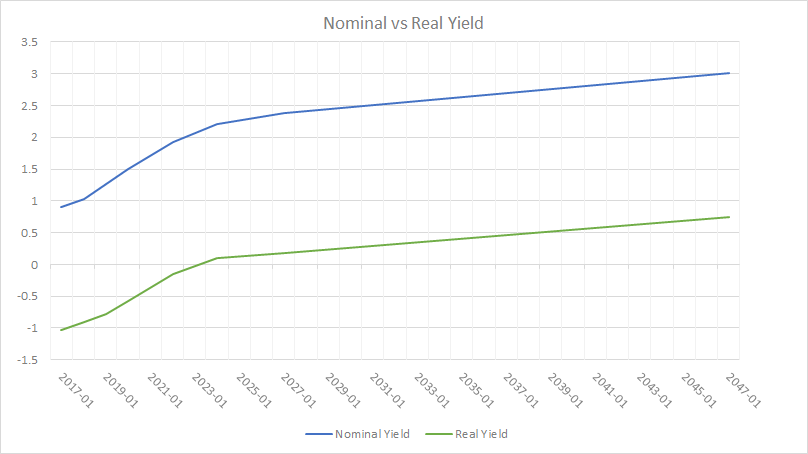
\includegraphics[scale=0.75]{graphics/realvsnominal.png}
		\caption{Wykresy struktury terminowej stopy procentowej w ujęciu nominalnym i rzeczywistym.}
	\end{figure}

	Kalibracja krzywej nominalnej dla US CPI ZC Bond na dzień 2017-04-01 (dane Reuters) oraz US Gov Yield Curve na dzień 2017-04-01.
	
\chapter*{Podsumowanie}

Rynek produktów linkowanych do inflacji jest częścią gospodarki szybko rozwijającą się oraz odpowiada na potrzebę instytucji efektywnie i racjonalnie zarządzających ryzykiem finansowym. Instrumenty finansowe powiązane z inflacją są ważne w szczególności dla instytucji, które identyfikują ryzyko inflacyjne w procesie zarządzania ryzykiem: fundusze emerytalne, fundusze Private Equity, hedgingowe, banki państwowe i komercyjne oraz spółki skarbu państwa

Podstawą zrozumienia i przeprowadzenia wyceny instrumentów pochodnych powiązanych z inflacją jest teoria modelowania stóp procentowych bazująca na ujęciu modelowania w świecie krzywych nominalnych oraz rzeczywistych. W pracy został opisany sposób podejścia do modelowania inflacji oraz konstrukcji krzywych projekcyjnych indeksu zmiany cen a także najważniejszy z modeli wyceny instrumentów powiązanych z inflacją - model Jarrowa i Yildirim. Stanowi on punkt wyjścia do budowy innych modeli wycen instrumentów inflacyjnych. 

Bazowym instrumentem zapewniającym zabezpieczenie przed ryzykiem inflacji jest obligacja indeksowana do inflacji. Ponadto na rynku dostępne są także instrumenty pochodne powiązane z procesem inflacji:
\begin{itemize}
	\item swap zerokuponowy,
	\item swap Year-on-Year,
	\item opcje cap oraz floor.
\end{itemize}
W pracy zostały wyprowadzone wzory na wartości wycen wyżej wymienionych kontraktów w modelu Jarrowa i Yildirima a także przedstawione ceny bazujące na danych dostępnych na rynku. 

Motywację do podjęcia tematu modelowania inflacji i instrumentów pochodnych indeksowanych do inflacji stanowił fakt, że na rynku polskim instrumenty te są mało znane i niezrozumiałe. Powyższa praca ta jest pierwszą opisującą aparat matematyczny i podejście do modelowania w języku polskim.

\begin{thebibliography}{11}
	\bibitem[1]{1} N. Belgrade, E. Benhamou, \emph{Smart Modeling of the Inflation Market: Taking into Account the Seasonality , Risk Magazine, Inflation Risk}, Risk Magazine, Inflation Risk, Supplement, 2004.
	
	\bibitem[2]{2} M. Hinnerich, \emph{Inflation indexed swaps and swaptions}, Journal of Banking and Finance, 2008.
	
	\bibitem[3]{3} R. Jarrow, Y. Yildirim, \emph{Pricing Treasury Inflation Protected Securities and Related Derivatives using an HJM Model}, Journal of Financial and Quantitative Analysis 38(2), 2003, 409-430.
	
	\bibitem[4]{4}	F. Mercurio, \emph{Pricing Inflation-Indexed Derivatives}, Quantitative Finance, 2005.
	
	\bibitem[5] {5}F. Mercurio, N. Moreni, \emph{Inflation with a smile.} Risk March, Vol. 19(3), 2006, 70-75.
	
	\bibitem[6] {6}J. Jakubowski , A. Palczewski, M. Rutkowski, Ł. Stettner,  \emph{Matematyka finansowa}, WNT, Warszawa, 2003.
	
	\bibitem[7] {7} D. Brigo, F. Mercurio, \emph{Interest Rate Models: Theory and Practice}, 2nd Ed., Springer, Berlin Heidelberg, 2006.
	
	\bibitem[8] {8} N.G. Mankiw, M.P.Taylor, \emph{Makroekonomia}, PWE, Warszawa, 2009.
	
		
\end{thebibliography}


\end{document}
